\chapter{补体系统}
\begin{framed}
    \noindent\textbf{【知识体系】}
\begin{center}
    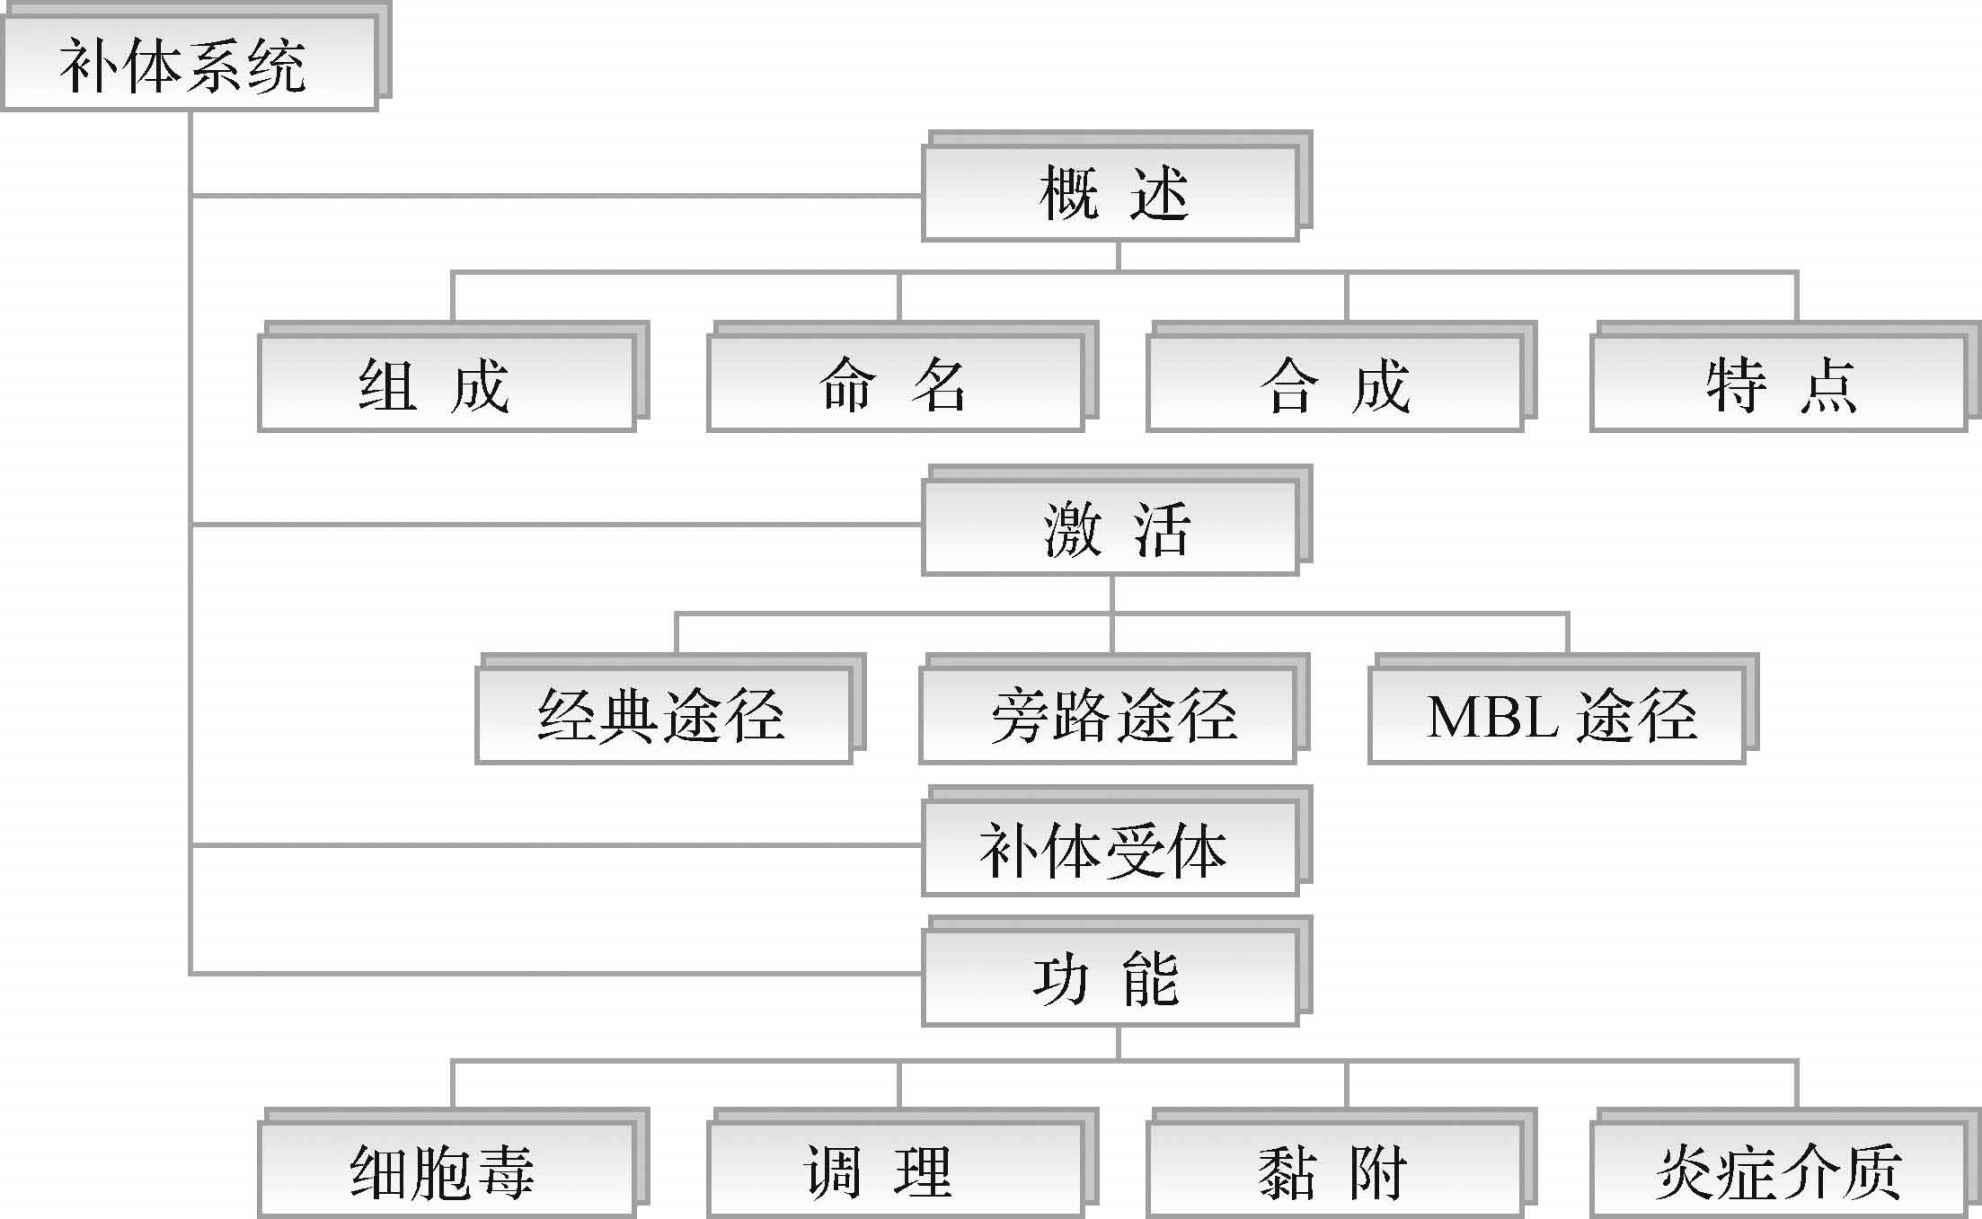
\includegraphics[width=0.6\textwidth]{./images/Image00078.jpg}
\end{center}

\noindent\textbf{【课前思考】}

机体中有哪种成分能辅助抗体的作用?能增强吞噬细胞的吞噬作用?能介导免疫细胞的游走?为什么机体健康时不会导致活化而在炎症时会产生活化作用?

\noindent\textbf{【本章重点】}

1.补体的概念、组成、特点;

2.补体激活的三条途径及生物学意义。

\noindent\textbf{【教学目标】}

1.掌握补体的概念、组成、特点;

2.掌握补体三条激活途径(经典途径、替代途径、MBL途径)的主要异同点;

3.掌握补体激活的生物学作用。
\end{framed}

在血液或体液内除Ig分子外,还发现另一族参与免疫效应的大分子,称为补体分子。早在19世纪末,发现在新鲜免疫血清内加入相应细菌,无论进行体内或体外实验,均证明可以将细菌溶解,将这种现象称之为免疫溶菌现象。如将免疫血清加热60℃、30min则可丧失溶菌能力。进一步证明免疫血清中含有两种物质与溶菌现象有关,即对热稳定的组分称为杀菌素,即抗体。其后又证实了抗各种动物红细胞的抗体加入补体成分亦可引起红细胞的溶解现象。自此建立了早期的补体概念,即补体为正常血清中的单一组分,它可被抗原与抗体形成的复合物所活化,产生溶菌和溶细胞现象。而单独的抗体或补体均不能引起细胞溶解现象。

补体(complement,C)是存在于人和动物正常新鲜血浆中具有酶样活性的一组不耐热的球蛋白。补体系统是30余种广泛存在于血清、组织液和细胞膜表面蛋白质组成的、具有精密调控机制的蛋白质反应系统,其活化过程表现为一系列丝氨酸蛋白酶的级联酶解反应。多种微生物成分、抗原抗体复合物以及其他外源性或内源性物质可通过3条既独立又交叉的途径激活补体,活化的产物具有调理吞噬、杀伤细菌/细胞、溶解病毒、介导炎症、调节免疫应答和溶解清除免疫复合物等多种生物学功能。补体不仅是机体天然免疫防御的重要部分,也是抗体发挥免疫效应的主要机制之一,并对免疫系统的功能具有调节作用。补体缺陷、功能障碍或过度活化与多种疾病的发生和发展过程密切相关。

\section{概述}


\subsection{补体系统的组成}

补体系统由补体固有成分、补体受体、血浆及细胞膜补体调节蛋白等组成。

1.补体固有成分:又称补体成分(complement
component),是存在于血浆及体液中、构成补体基本组成的蛋白质,包括:经典激活途径的C1q、C1r、C1s、C2、C4;旁路激活途径的B因子、D因子和备解素(properdin,P因子);甘露聚糖结合凝集素激活途径(MBL途径)的MBL、MBL相关丝氨酸酶(MASP);补体活化的共同组分C3、C5、C6、C7、C8、C9。

2.补体受体(complement
receptor):指存在于不同细胞膜表面、能与补体激活过程中形成的活性片段相结合、介导多种生物效应的受体分子。目前已发现的补体受体包括:CR1、CR2、CR3、CR4、CR5及C3aR、C4aR、C5aR、C1qR、C3eR、H因子受体(HR)等。

3.补体调节蛋白(complement regulatory
proteins):指存在于血浆中和细胞膜表面,通过调节补体激活途径中关键酶而控制补体活化强度和范围的蛋白分子,包括:血浆中H因子、I因子、C1-INH、C4bp、S蛋白、Sp40/40、羧肽酶N(过敏毒素灭活因子)、H因子样蛋白(FHL)、H因子相关蛋白(FHR);存在于细胞膜表面的衰变加速因子(DAF)、膜辅助蛋白(MCP)、CD59等。


\subsection{补体的命名}

(一)补体成分的命名

补体经典激活途径和终末成分按照其发现先后,依次命名为C1、C2、C3~C9,但其激活次序却为C1-C4-C2-C3-C5-C6-C7-C8-C9。补体旁路途径成分称为因子(factor),并以字母相区别,如B因子、D因子、H因子、I因子、P因子。

(二)补体片段的命名

补体在活化过程中被裂解成多个片段,其中较小的片段为a(如C3a、C5a),较大者为b(如C3b),但C2例外,C2a为较大片段。另外,失活的C3b和C4b还可继续裂解为较小片段,如C3c、C3d等。

(三)其他命名原则

此外,补体还有其他命名原则:①组成某一补体成分的肽链用希腊字母表示,如C3α链和β链等;②具有酶活性的分子,在其上以横线表示,如C1为无酶活性分子,而Cī为有酶活性分子;③补体调节蛋白可按其功能命名,如衰变加速因子(DAF)、膜辅助蛋白(MCP)等。


\subsection{补体的合成}

约90\%血浆补体成分由肝脏合成,仅少数成分在肝脏以外的其他部位合成。例如:C1由肠上皮细胞和单核/巨噬细胞产生;D因子在脂肪组织中产生。此外,多种器官和细胞(如单核/巨噬细胞、内皮细胞、淋巴细胞、神经胶质细胞、肾脏上皮细胞、生殖器官等)也能合成补体成分。

IFN-γ、IL-1、TNF-α、IL-6、IL-11等细胞因子可刺激补体基因转录和表达。感染部位浸润的单核/巨噬细胞可产生全部补体成分,从而及时补充和提高局部补体水平。因此,在组织损伤急性期以及炎症状态下,补体产生增多,血清补体水平升高。


\subsection{补体的生物学特点}

1.含量相对稳定:约占血浆总球蛋白的10\%~15\%,不因免疫而增强。

2.对理化因素的作用敏感:61℃、2min,56℃、15~30
min灭活;而抗体能耐受56℃、30
min。保存在-20℃以下,0~10℃活性3~4天。对其他理化因素,如紫外线、震荡、酸、碱等都敏感。

3.能与抗原抗体复合物结合并被激活。补体激活后,导致一系列生物活性反应,增强机体防御能力,协助抗体消灭病原微生物。

4.不同种动物血清中补体含量不一致。豚鼠中补体含量最多,成分最强,活性最强。

5.代谢率高。合成率:0.5~1.5mg/kg、h,半衰期58小时。

\section{补体系统的激活}

血浆中非活化的补体成分无生物学功能,仅当补体级联酶促反应被激活后,才产生具有生物学活性的产物。多种外源性或内源性物质可通过三条途径激活补体:

\begin{figure}[!htbp]
 \centering
 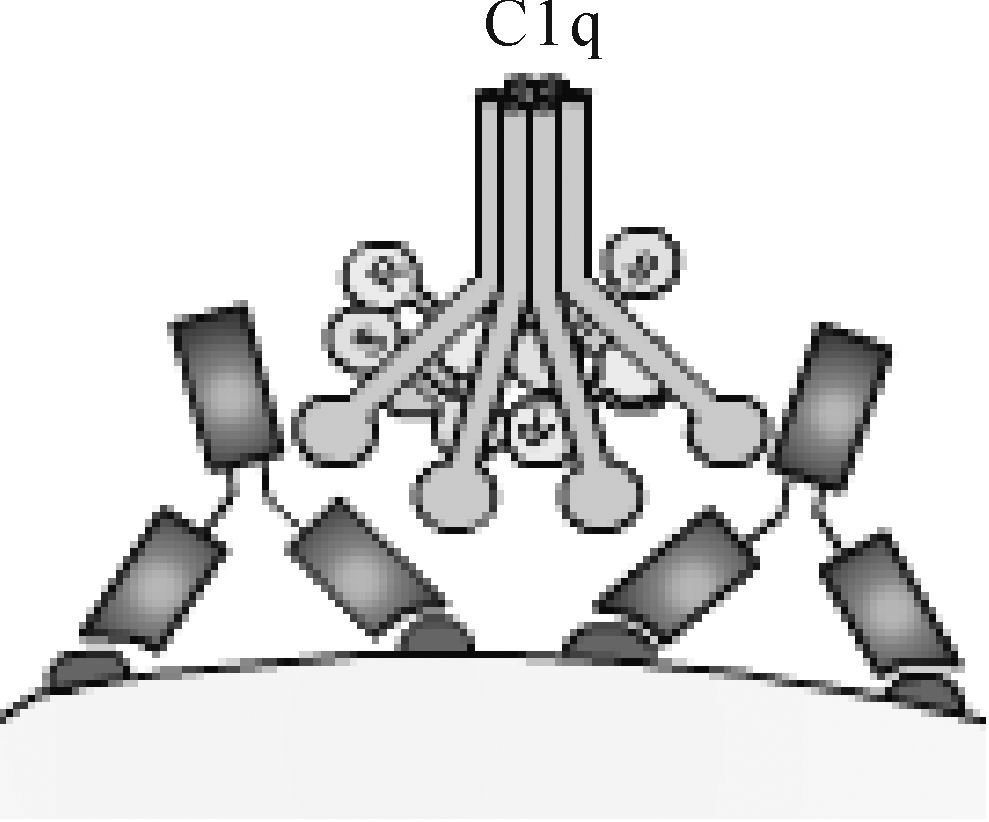
\includegraphics{./images/Image00079.jpg}
 \captionsetup{justification=centering}
 \caption{抗原抗体激活物激活C1q}
 \label{fig5-1}
  \end{figure} 

①从C1q-C1r2-C1s2开始的经典途径(classic
pathway),抗原-抗体复合物为主要激活物(图\ref{fig5-1});

②从C3开始的旁路途径(alternative pathway),其不依赖于抗体;

③通过甘露聚糖结合凝集素(mannan binding
lectin,MBL)糖基识别的凝集素激活途径(MBL
pathway)。此外,上述三条途径有共同的终末反应过程。


\subsection{经典途径}

1.激活物:

(1)IgM或IgG的抗原抗体复合物。

(2)核酸、酸性粘多糖、肝素、鱼精蛋白、C-反应蛋白、细菌脂多糖(LPS)、某些病毒蛋白(如HIV的gp120等)等。

2.其活化过程分为3个功能单位:

(1)识别单位:C1q、C1r、C1s

(2)活化单位:C4、C2、C3

(3)攻膜单位:C5~C9

(一) 参与经典途径的补体成分

参与经典途径活化的补体成分依次为:C1、C4、C2、C3、C5、C6、C7、C8、C9。

血浆中C1通常以C1q(C1r)2
(C1s)2复合大分子形式存在,每个C1s和C1r分子均含一个丝氨酸蛋白酶结构域,如图\ref{fig5-2}所示。

\begin{figure}[!htbp]
 \centering
 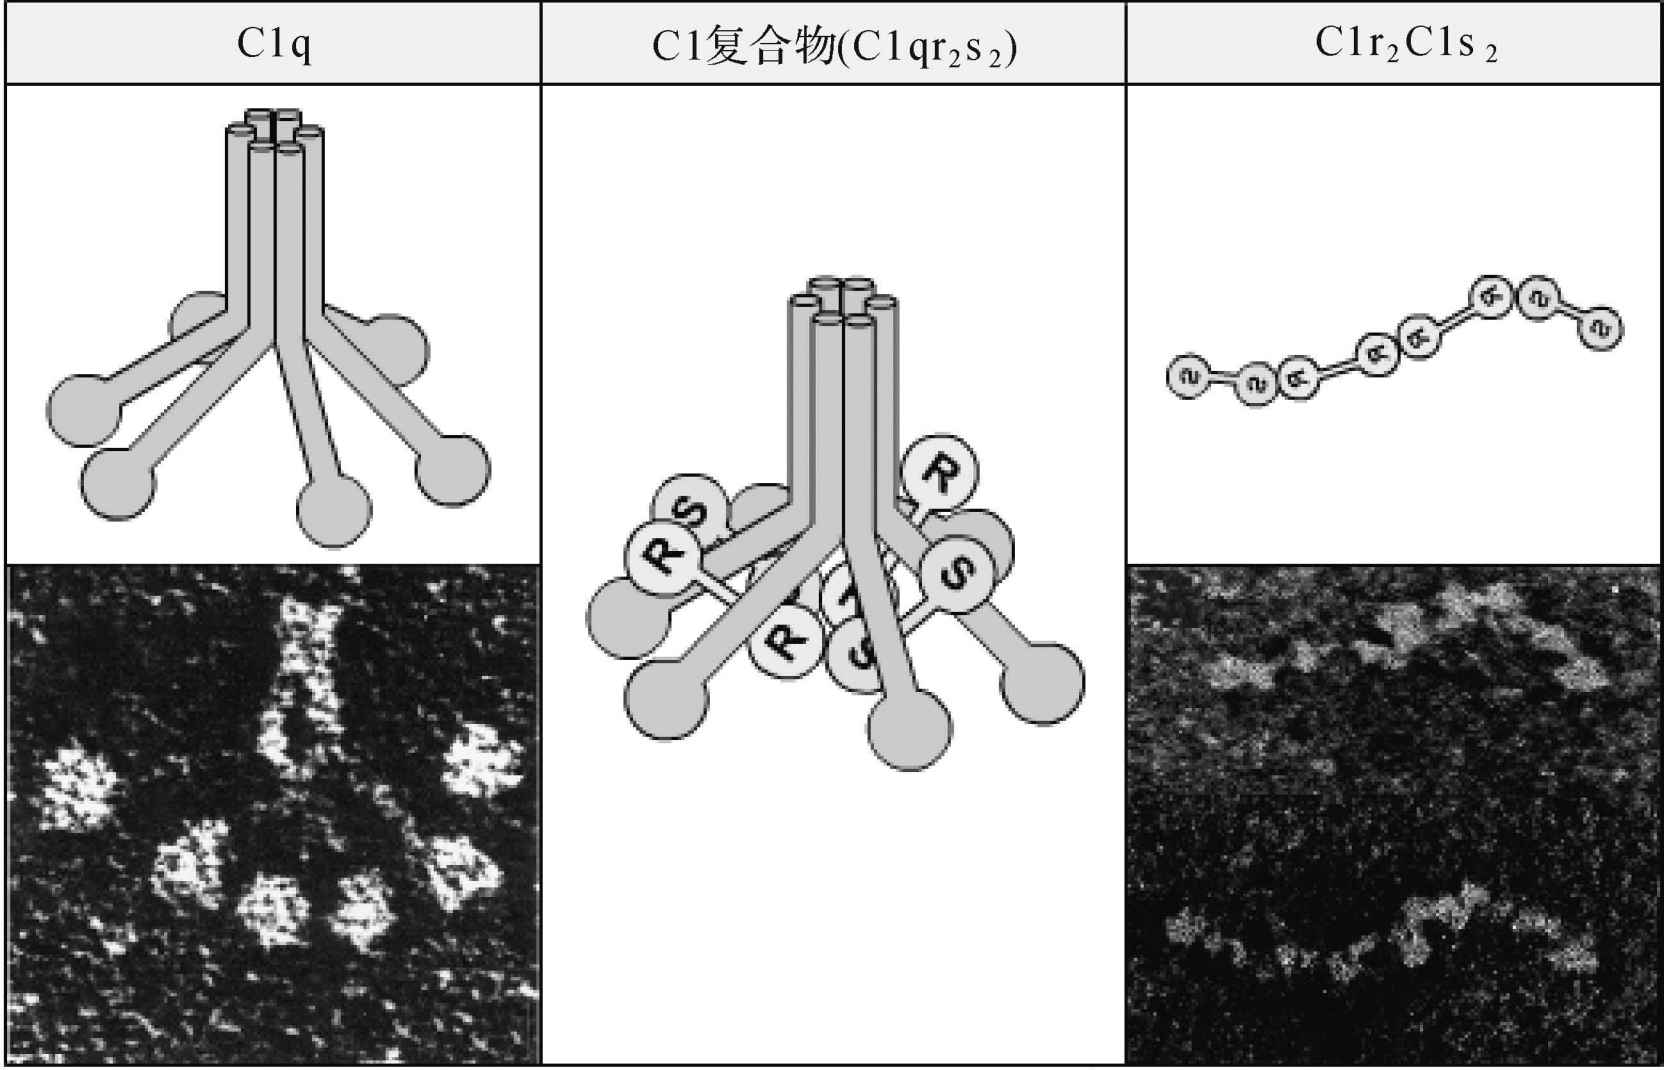
\includegraphics[width=0.6\textwidth]{./images/Image00080.jpg}
 \captionsetup{justification=centering}
 \caption{C1分子结构模式图}
 \label{fig5-2}
  \end{figure} 

C2为丝氨酸蛋白酶原,其血浆浓度很低,是补体活化级联酶促反应的限速步骤。C3是血浆中浓度最高的补体成分,是3条补体激活途径的共同组分。C3分子由α、β两条多肽链组成。C4由α、β和γ三条肽链组成,其分子结构与C3相似。

最终形成膜攻击复合物,造成靶细胞膜的损伤和靶细胞溶解。C5转化酶裂解C5形成的C5b可依次结合C6、C7,形成C5b67复合物并结合在细胞膜表面。C8可结合该复合物中的C7,进而通过构型改变插入细胞膜脂质双层,使形成的C5b678复合物牢固地附着在细胞表面,并使细胞膜出现轻微损伤,但其溶细胞能力有限。当附着在细胞膜表面的C5b678复合物与C9分子结合,聚合12~15个单链的C9分子形成C5b~9复合物,才可在细胞膜上形成孔道。因此,C5b~9称为膜攻击复合物(MAC)。电镜下可见到这种聚合C9分子是一个中空的多聚体,插入靶细胞的脂质双层膜后可造成细胞膜上内径为11nm的小孔,导致细胞内容物外漏,最终导致靶细胞溶解破坏。

(二)经典途径活化过程

补体经典途径激活过程如图\ref{fig5-3}所示。

\begin{figure}[!htbp]
 \centering
 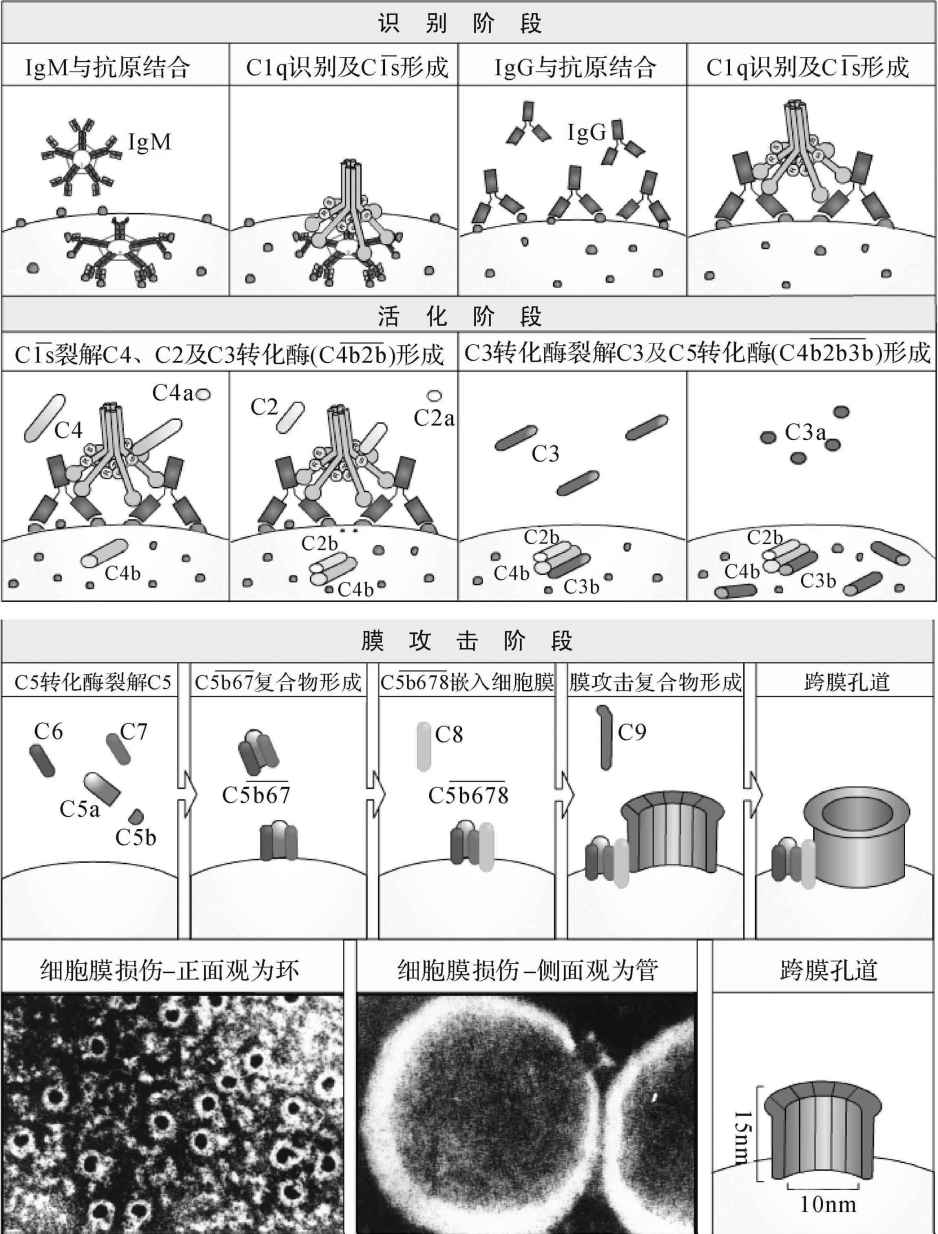
\includegraphics[width=0.7\textwidth]{./images/Image00081.jpg}
 \captionsetup{justification=centering}
 \caption{补体经典途径激活过程模式图}
 \label{fig5-3}
  \end{figure} 

1.识别阶段:当抗体与抗原结合后,抗体构象发生改变,暴露出位于Fc段上的补体结合点,Clq便与之结合。继而激活Clr、C1s。

C1q须与2个以上Fc段结合后才发生构型改变,使与C1q非共价结合的两分子C1r相互裂解而活化,活化的C1r激活C1s的丝氨酸蛋白酶活性。

C1s的第一个底物是C4分子:在Mg\textsuperscript{2+}
存在下,C1s使C4裂解为C4a小片段和C4b大片段,大部分新生的C4b与H\textsubscript{2}
O反应而失活,仅5\% C4b共价结合至紧邻细胞或颗粒表面。

C1s的第二个底物是C2分子:C2与C4b形成Mg\textsuperscript{2+}
依赖性复合物,被CIs裂解后产生C2b大片段和C2a小片段。C2b与C4b结合成C4b2b复合物(即C3转化酶)。丝氨酸蛋白酶活性存在于C2b片段,其活性仅在与C4b结合时显示。

2.活化阶段:活化的C1s依次裂解C4和C2,形成具有酶活性的C3转化酶,后者进一步酶解C3并形成C5转化酶。此过程为经典途径的活化阶段。在活化阶段,补体C4、C2、C3和C5的级联酶解中,每一补体分子均裂解为a、b两个片段。a片段为小分子,游离于体液中,发挥趋化作用、过敏毒素和免疫黏附、调理作用等;b片段为大分子,结合在激活物颗粒(如细胞、细菌)表面,参与C3转化酶和C5转化酶的形成。

3、膜攻击阶段:C5转化酶(C3bBb3b或C4b2a3b)将C5裂解为小片段C5a和大片段C5b;C5a游离于液相,是重要的炎症介质;C5b可与C6稳定结合为C5b6;C5b6自发与C7结合成C5b~7,暴露膜结合位点,与附近的细胞膜非特异性结合;结合在膜上的C5b~7可与C8结合,所形成的C5b~8可促进C9聚合,形成C5b6789n复合物,即膜攻击复合物(membrane
attack
complex,MAC)。插入膜上的MAC通过破坏局部磷脂双层而形成“渗漏斑”,或形成穿膜的亲水性孔道,最终导致细胞崩解。


\subsection{旁路途径}

旁路途径又称替代激活途径(alternative
pathway),指由B因子、D因子和备解素参与,直接由微生物或外源异物激活C3,形成C3与C5转化酶,激活补体级联酶促反应的活化途径。旁路途径是最早出现的补体活化途径(图\ref{fig5-4}),乃抵御微生物感染的非特异性防线。

\begin{figure}[!htbp]
 \centering
 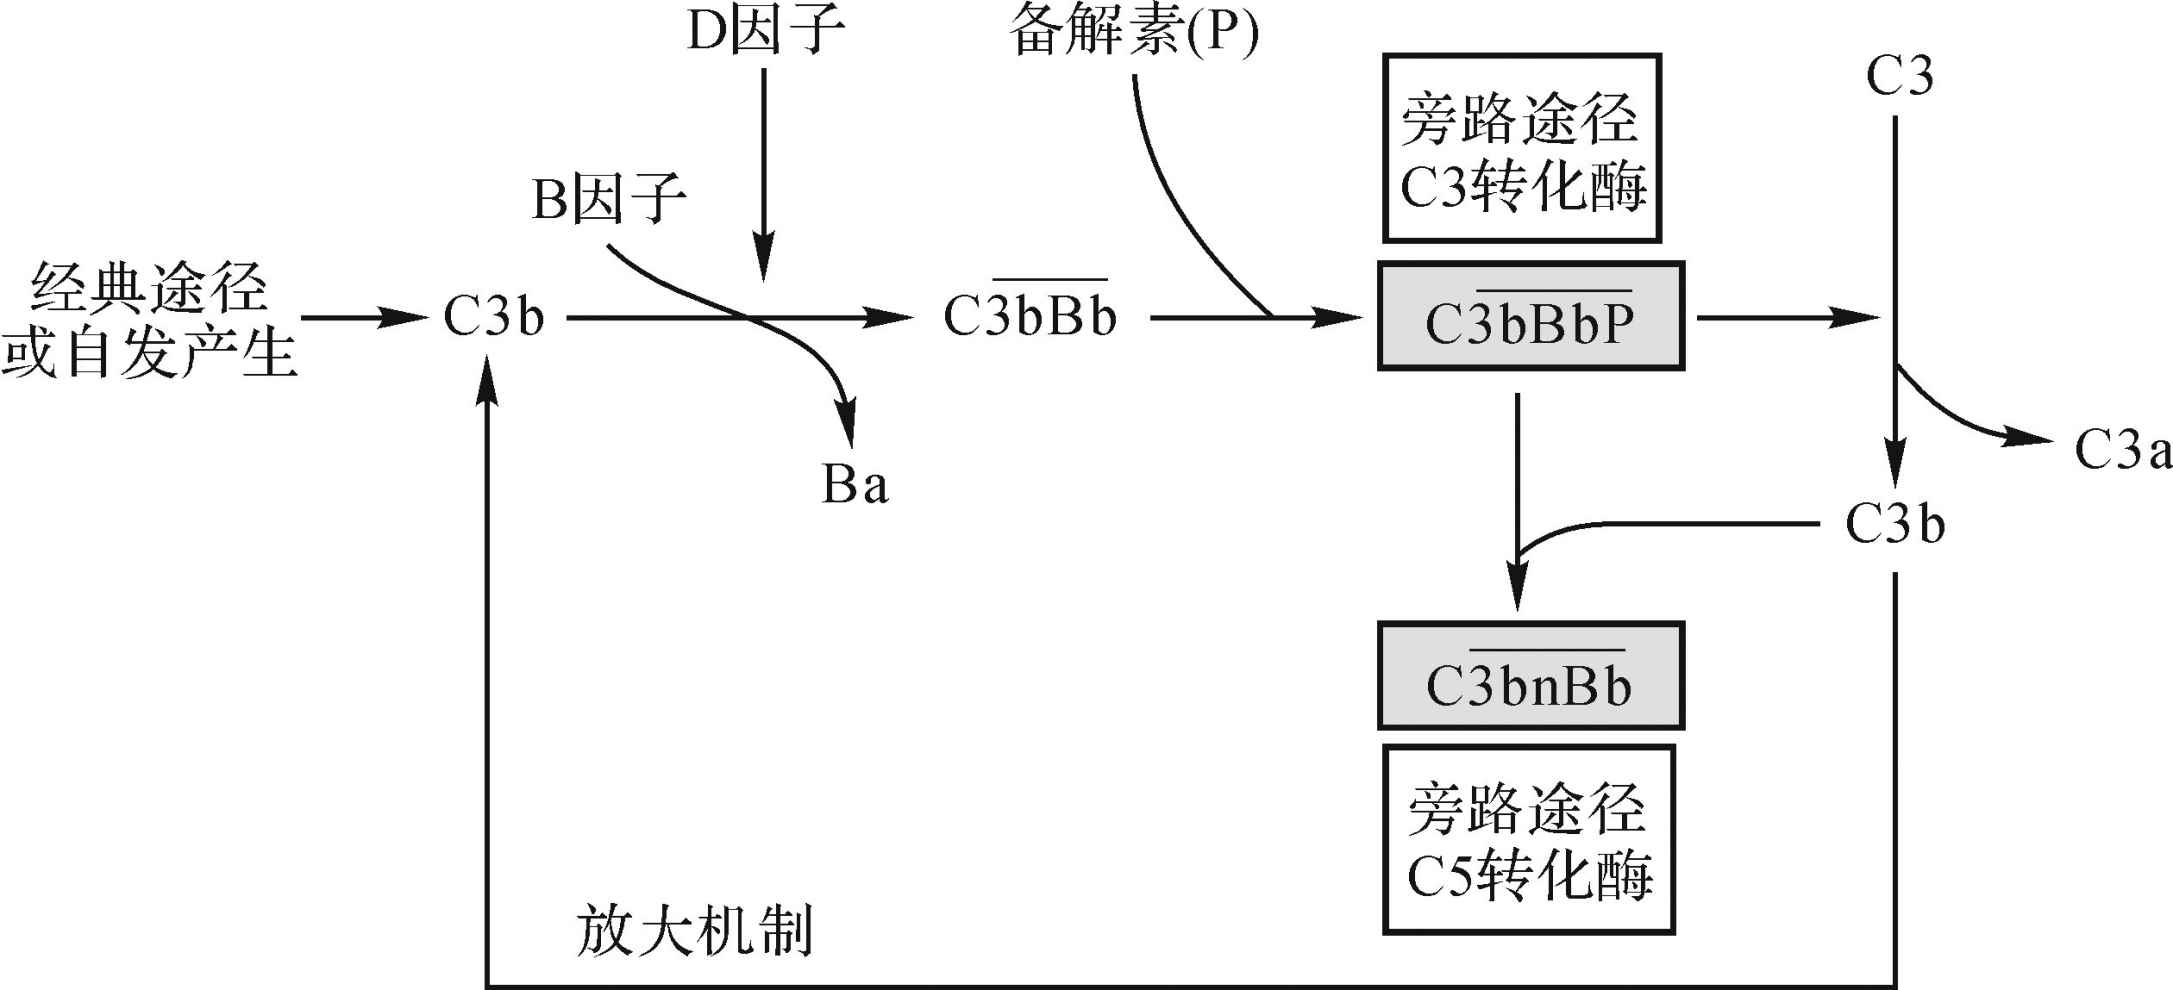
\includegraphics{./images/Image00082.jpg}
 \captionsetup{justification=centering}
 \caption{旁路途径示意图}
 \label{fig5-4}
  \end{figure} 

(一) 旁路途径的主要激活物

旁路途径的“激活物”乃为补体激活提供保护性环境和接触表面的成分,如某些细菌、内毒素、酵母多糖、葡聚糖等。

(二)旁路途径活化过程

1.参与成分:C3、C5~C9、B因子、D因子、P因子。

2.激活过程:不需要C1、C4、C2参与,血浆中天然的C3能缓慢分裂成C3b是关键。

C3有限裂解和C3bB形成。正常情况下,体内的蛋白水解酶可使C3有限微弱裂解,产生少量C3b,使机体总保持着“箭在弦上,一触即发”的警觉状态。处于液相的C3b极不稳定,易被体液中的I因子、H因子灭活。一旦有病原微生物入侵,细菌细胞壁的脂多糖和肽聚糖等激活物提供了补体分子可以接触的固相表面,使补体级联反应得以进行。C3b结合在细菌表面后,可发生结构改变,结合B因子,形成稳定的C3bB复合物,并在D因子作用下,进一步裂解B因子形成替代途径的C3转化酶,触发替代途径的激活。

与激活物表面结合的C3bBb可裂解更多C3分子,其中部分新生的C3b又可与Bb结合,此即旁路激活的正反馈放大效应。少量C3b与C3bBb复合物中的C3b结合,形成C5转化酶C3bnBb,其后为终末过程(图\ref{fig5-5})。

\subsection{MBL途径}

MBL途径(MBL pathway)指由血浆中甘露聚糖结合的凝集素(mannan binding
lectin,MBL)
直接识别多种病原微生物表面的N-氨基半乳糖或甘露糖,进而依次活化MASP-1、MASP-2、C4、C2、C3,形成和经典途径相同的C3与C5转化酶,激活补体级联酶促反应的活化途径。MBL激活途径的主要激活物为含有N-氨基半乳糖或甘露糖基的病原微生物。
\begin{figure}[!htbp]
    \centering
    \begin{minipage}[b]{0.45\textwidth} 
        \centering
        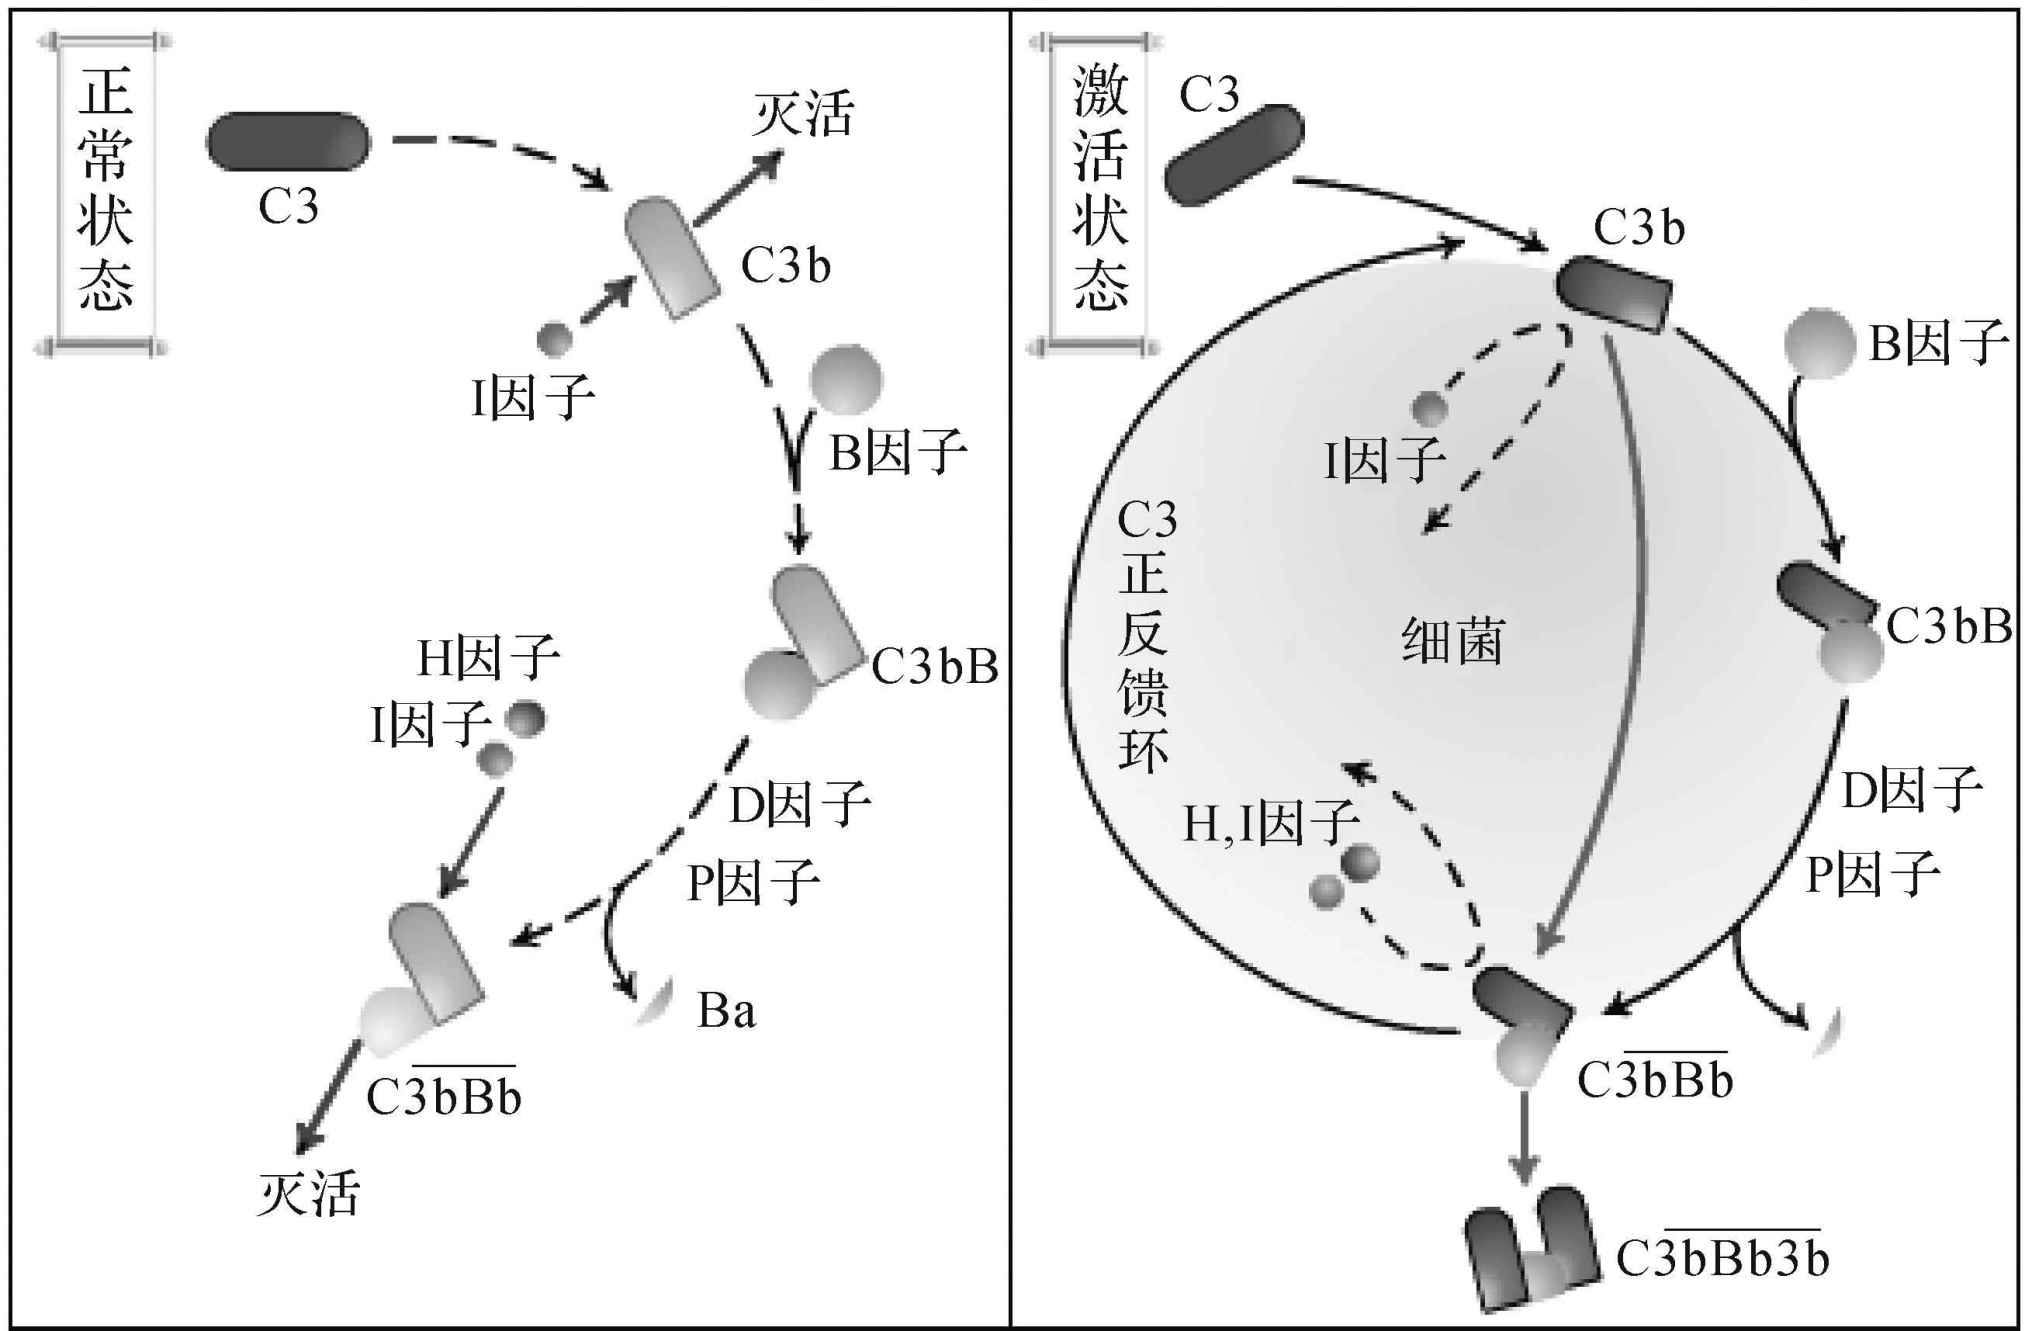
\includegraphics[height=.2\textheight]{./images/Image00083.jpg}
        \captionsetup{justification=centering}
        \caption{补体激活的旁路途径示意图}
        \label{fig5-5}
    \end{minipage}
%	\end{figure} 
	%\FloatBarrier
%\begin{figure}[!htbp]
%    \centering
\hspace{0.04\textwidth}%
\begin{minipage}[b]{0.45\textwidth} 
    \centering
    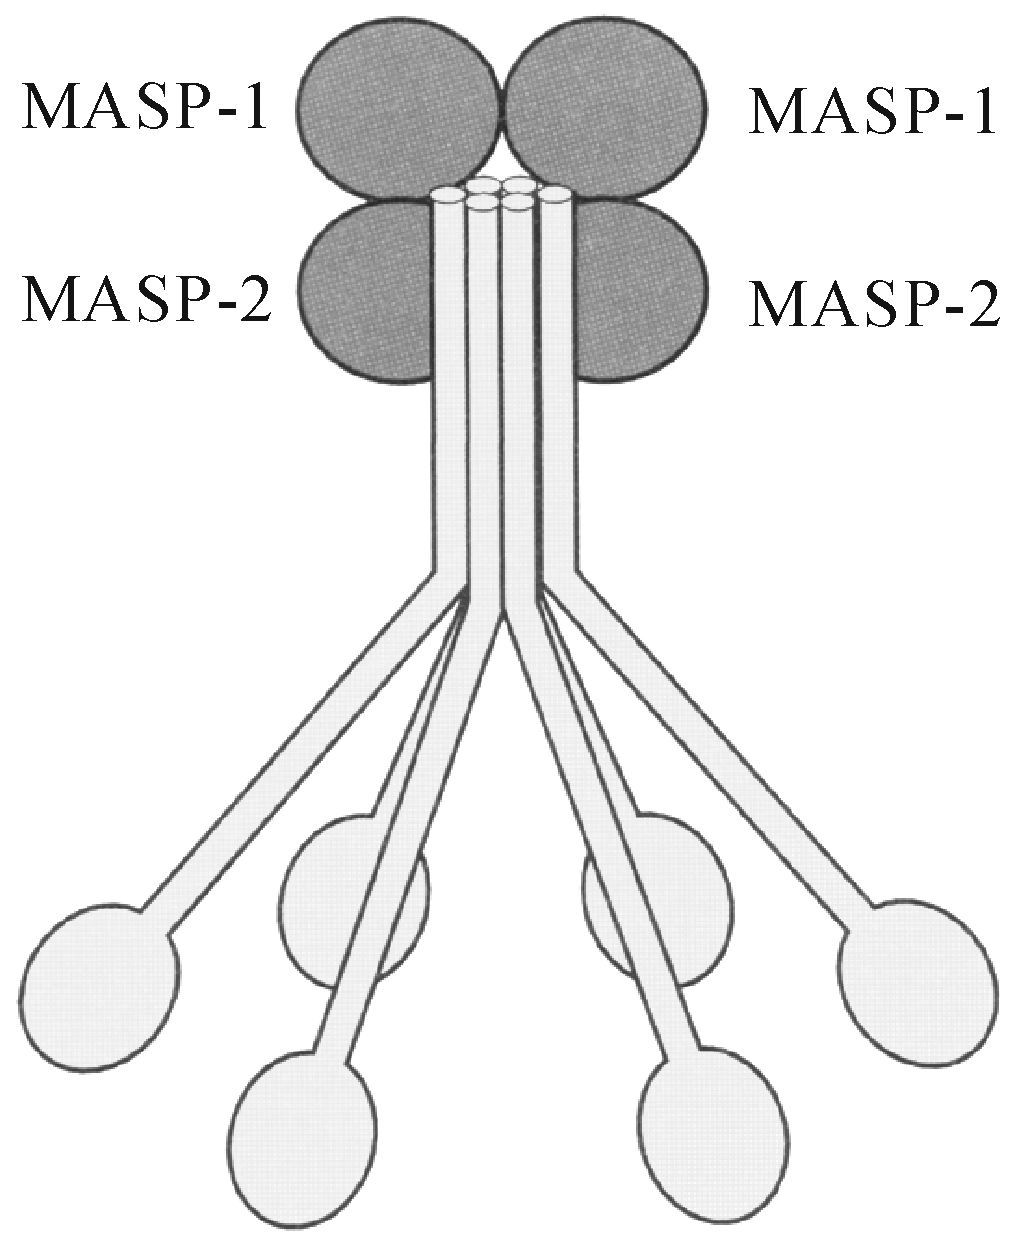
\includegraphics[height=.2\textheight]{./images/Image00084.jpg}
 \captionsetup{justification=centering}
 \caption{MASP结构示意图}
 \label{fig5-6}
\end{minipage}
\end{figure} 


MBL分子结构类似于C1q分子。依赖于Ca\textsuperscript{2+}
存在,MBL可与多种病原微生物表面的N-氨基半乳糖或甘露糖结合,并发生构型改变,导致MBL相关的丝氨酸蛋白酶(MBL-associated
serine protease,MASP)活化(图\ref{fig5-6})。

MASP有两类:活化的MASP-2能以类似于C1s的方式裂解C4和C2,生成类似经典途径的C3转化酶C4b2a,进而激活后续的补体成分;MASP-1能直接裂解C3生成C3b,形成旁路途径C3转化酶C3bBb,参与并加强旁路途径正反馈环路(图\ref{fig5-7})。因此,凝集素途径对补体经典途径和旁路途径活化具有交叉促进作用。

\begin{figure}[!htbp]
 \centering
 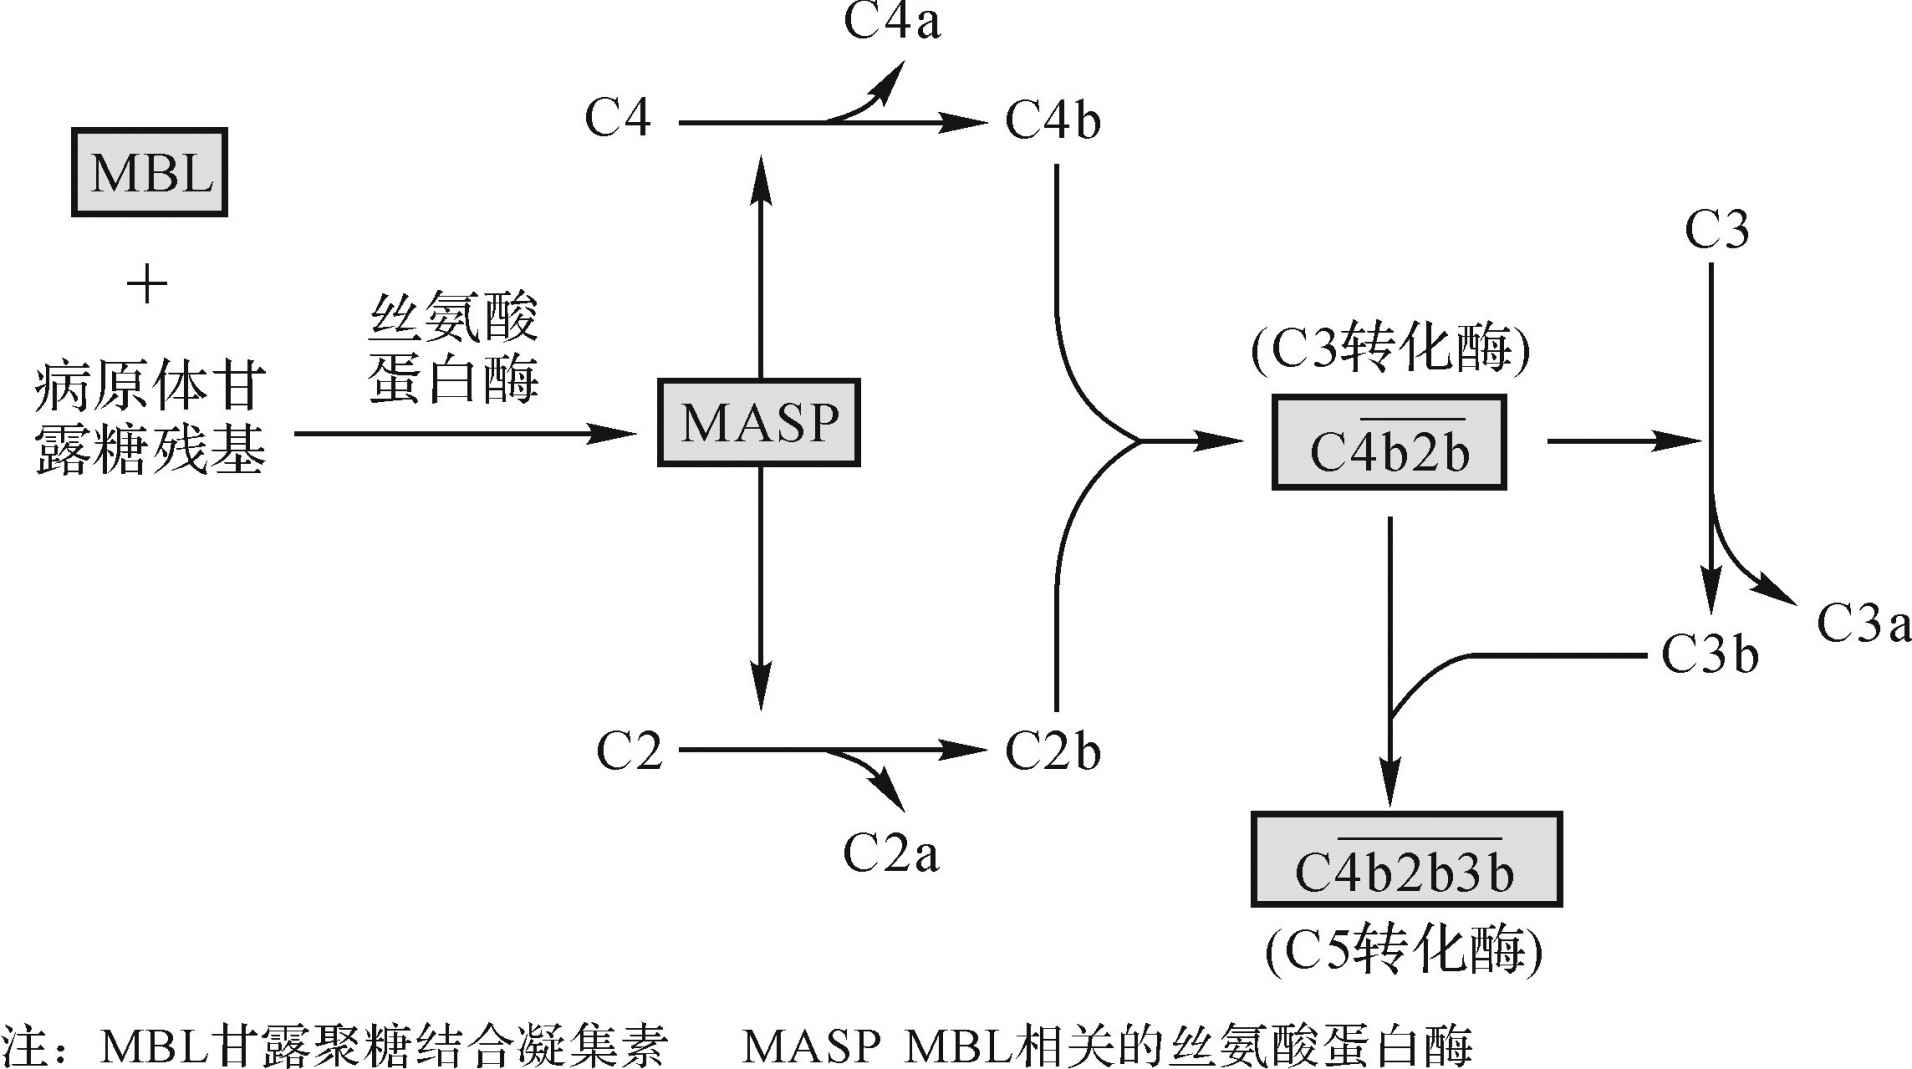
\includegraphics[width=.6\textwidth]{./images/Image00085.jpg}
 \captionsetup{justification=centering}
 \caption{补体激活的MBL途径}
 \label{fig5-7}
  \end{figure} 


\subsection{三条途径的比较}

补体激活的经典途径、旁路途径、MBL途径的区别见表\ref{tab5-1}。

\begin{longtable}[!t]{lp{4cm}p{4cm}p{4cm}}
    \caption{三条途径的区别}
    \label{tab5-1}\\
\toprule
比较项目 & 经典途径 & 旁路途径 & MBL途径\tabularnewline
\midrule
\endhead
激活物&抗原抗体复合物&细菌脂多糖等&病原微生物表面甘露糖残基\\
补体成分& C1~C9&B、D、P因子、C3、 C5~C9& MBL、MASP1,2、C2~C9\\
所需离子&Ca\textsuperscript{2+},Mg\textsuperscript{2+}&Mg\textsuperscript{2+}&Ca\textsuperscript{2+}\\
C3转化酶&C4b2b&C3bBb&C4b2b\\
C5转化酶&C4b2b3b&C3bnBb&C4b2b3b\\
作用&在特异性体液免疫应答的效应阶段发挥作用&参与非特异性免疫,在感染早期发挥作用&参与非特异性免疫,在感染早期发挥作用\\
\bottomrule
\end{longtable}

相同点:三条途径有共同的末端通路,即形成膜攻击复合物溶解细胞。三条激活途径全过程如图\ref{fig5-8}所示。

\begin{figure}[!t]
 \centering
 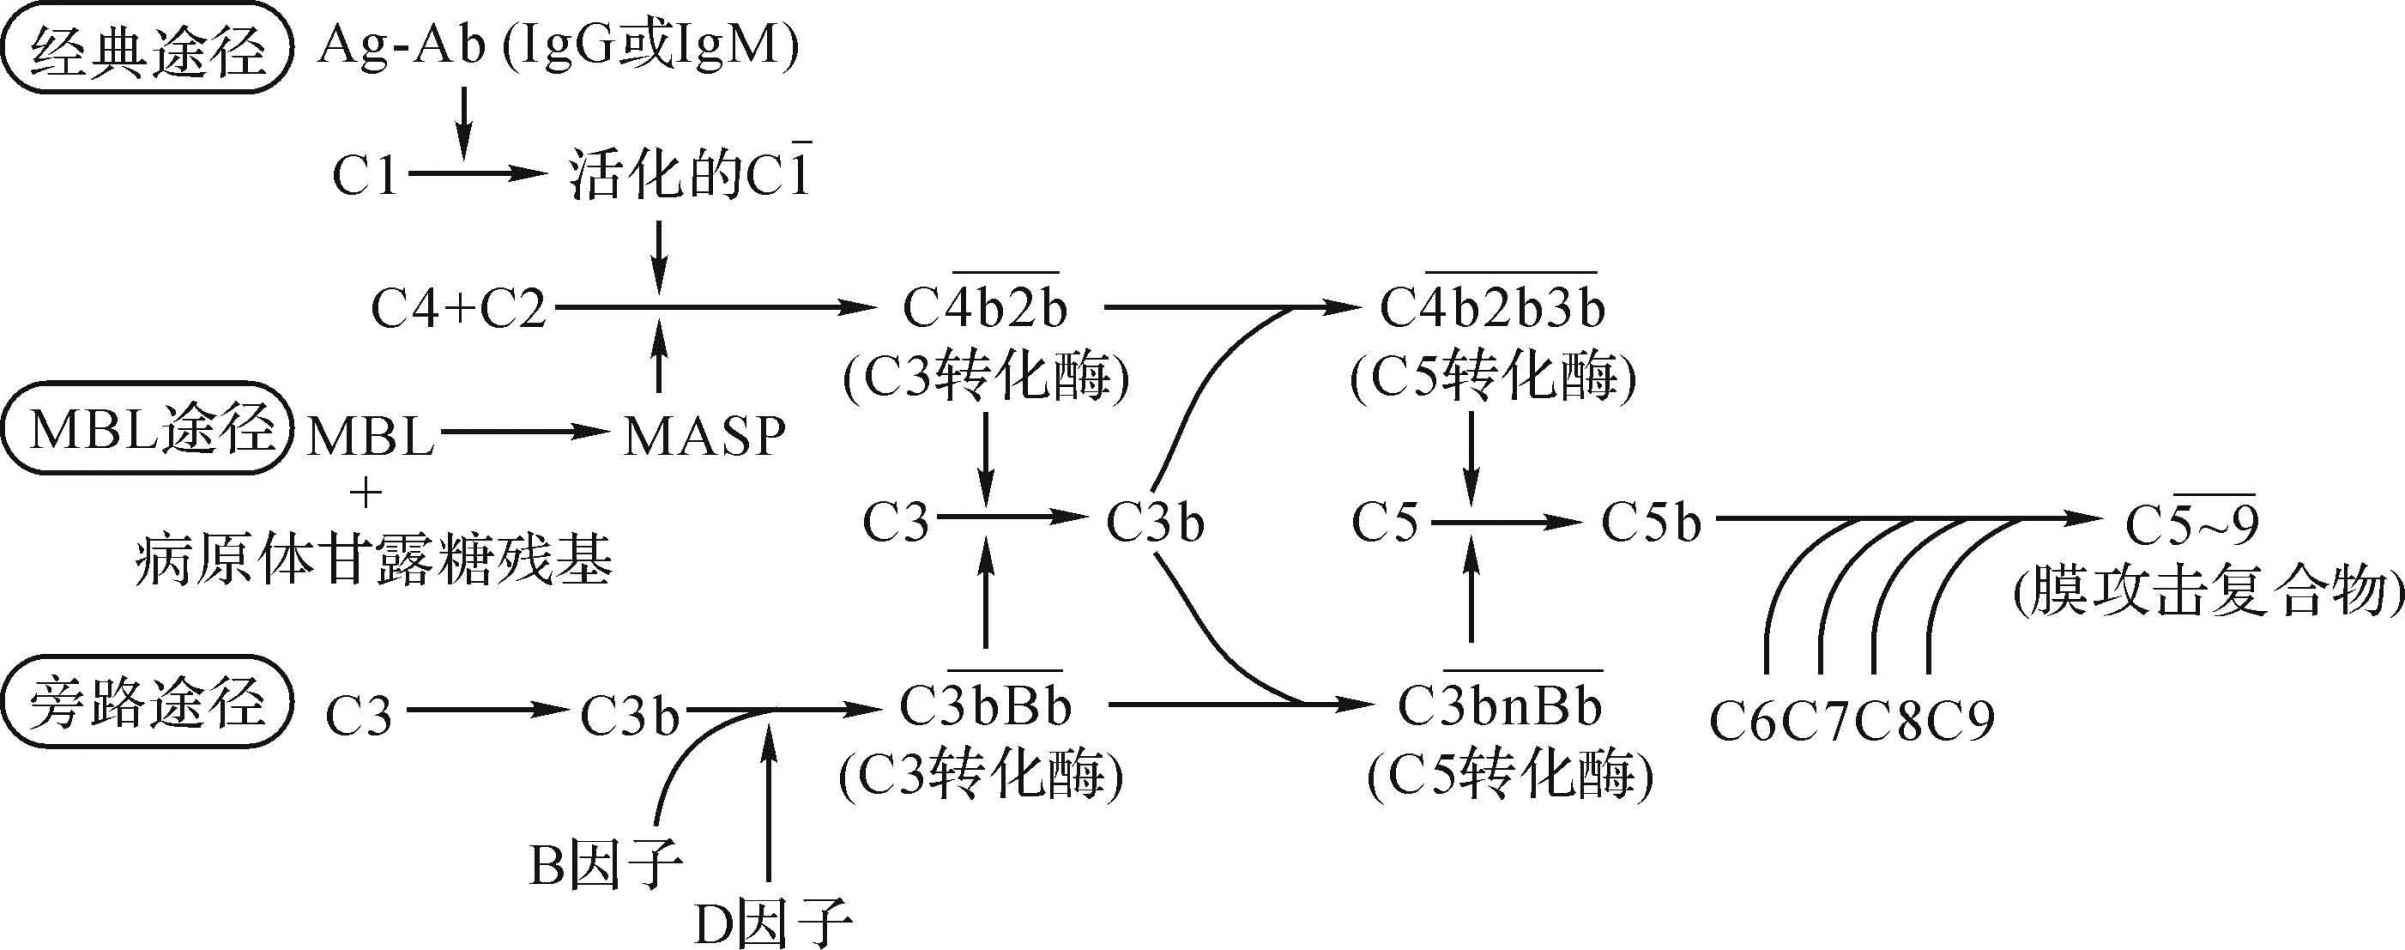
\includegraphics{./images/Image00086.jpg}
 \captionsetup{justification=centering}
 \caption{补体三条激活途径全过程示意图}
 \label{fig5-8}
  \end{figure} 

\section{补体受体}

补体活化过程中产生多种活性片段,它们通过与相应受体结合而发挥生物学效应。

(一)补体Ⅰ型受体(CR1,C3b受体,CD35)

CR1广泛分布于多种免疫细胞表面,血液中约85\%CR1表达于红细胞表面。CR1的配体依其亲和力为C3b、C4b、iC3b。

CR1的主要免疫学功能是:①调理作用:细菌或病毒表面的C3b可与吞噬细胞表面CR1结合,发挥调理作用;②调节补体活化:CR1可抑制C3转化酶活性,保护宿主细胞免受补体介导的损伤;③清除免疫复合物:红细胞借助CR1与吸附C3b的免疫复合物结合,将它们转移至肝、脾,由该处的巨噬细胞清除之。

(二)补体受体Ⅱ型(CR2,C3b受体,CD21)

CR2表达在B细胞、活化的T细胞、上皮细胞和滤泡树突状细胞(FDC)表面,其配体是iC3b、C3d、C3dg、C3b等。

CR2可与CD19和CD81在B细胞膜表面形成复合物,从而参与B细胞的激活。FDC表面的CR2可参与B细胞记忆的形成。此外,CR2可作为EBV进入B细胞或其他CR2阳性细胞的门户,从而参与某些疾病的发生和发展。

(三)补体受体Ⅲ型(CR3,Mac-1,CDHb/CD18)

CR3广泛分布于包括吞噬细胞在内的多种免疫细胞表面,其配体主要是iC3b。CR3可促进吞噬细胞吞噬iC3b包被的微生物颗粒。

(四)补体受体Ⅳ型(CR4,p150/95,CD11c/CD18)

CR4高表达于吞噬细胞表面,其配基和组织分布均与CR3相同。

(五)C5aR(CD88)和C3aR

C3aR和C5aR广泛表达于肥大细胞、嗜碱粒细胞、中性粒细胞、单核/巨噬细胞、内皮细胞、平滑肌细胞和淋巴细胞表面。C3a和C5a通过与相应受体结合而发挥作用。

(六)C1q受体

C1q受体可增强吞噬细胞对C1q调理的免疫复合物和MBL调理的细菌的吞噬作用,还可促进氧自由基产生、增强细胞介导的细胞毒作用等。

\section{补体的功能及生物学意义}

补体活化的共同终末效应是在细胞膜上组装MAC,介导细胞溶解效应。同时,补体活化过程中生成多种裂解片段,通过与细胞膜相应受体结合而介导多种生物功能。

\begin{figure}[!htbp]
 \centering
 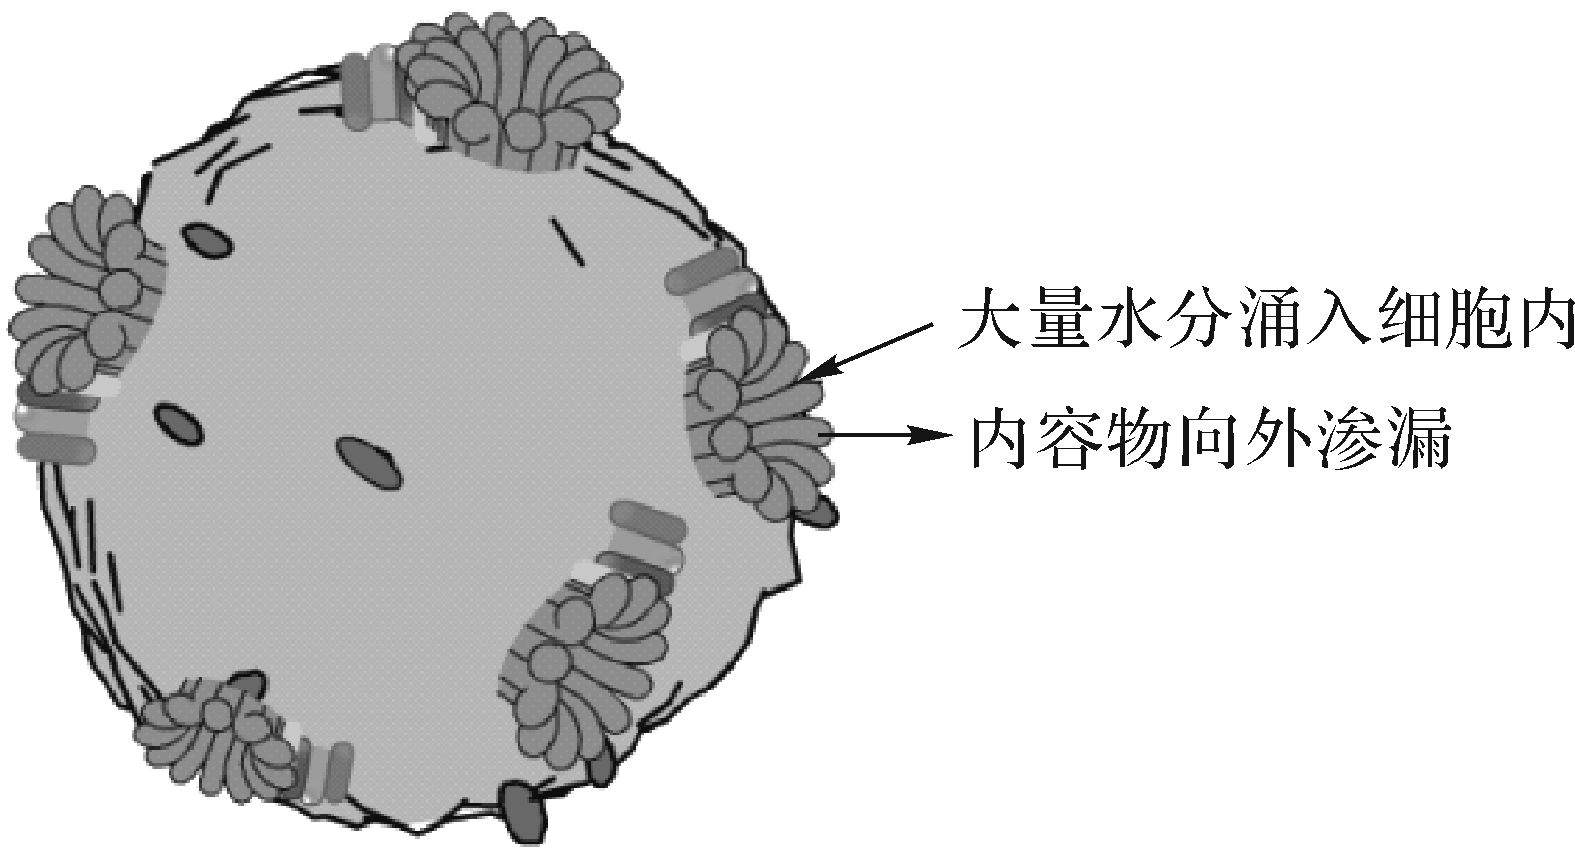
\includegraphics{./images/Image00087.jpg}
 \captionsetup{justification=centering}
 \caption{补体介导的细胞溶解}
 \label{fig5-9}
  \end{figure} 


\subsection{细胞毒及溶菌、溶解病毒作用}

补体激活产生MAC,形成穿膜的亲水性通道,破坏局部磷脂双层,最终导致细胞崩解。MAC的生物学效应是:溶解红细胞、血小板和有核细胞;参与宿主抗细菌(革兰阴性菌)和抗病毒(如HIV)防御机制。补体介导的细胞溶解如图\ref{fig5-9}所示。


\subsection{调理作用}

C3b、C4b和iC3b与细菌或其他颗粒结合,通过与吞噬细胞表面CR1、CR3、CR4结合而促进其吞噬作用,此为补体的调理作用。这种调理吞噬作用可能是机体抵抗全身性细菌和真菌感染的主要机制之一(图\ref{fig5-10})。

\begin{figure}[!htbp]
 \centering
 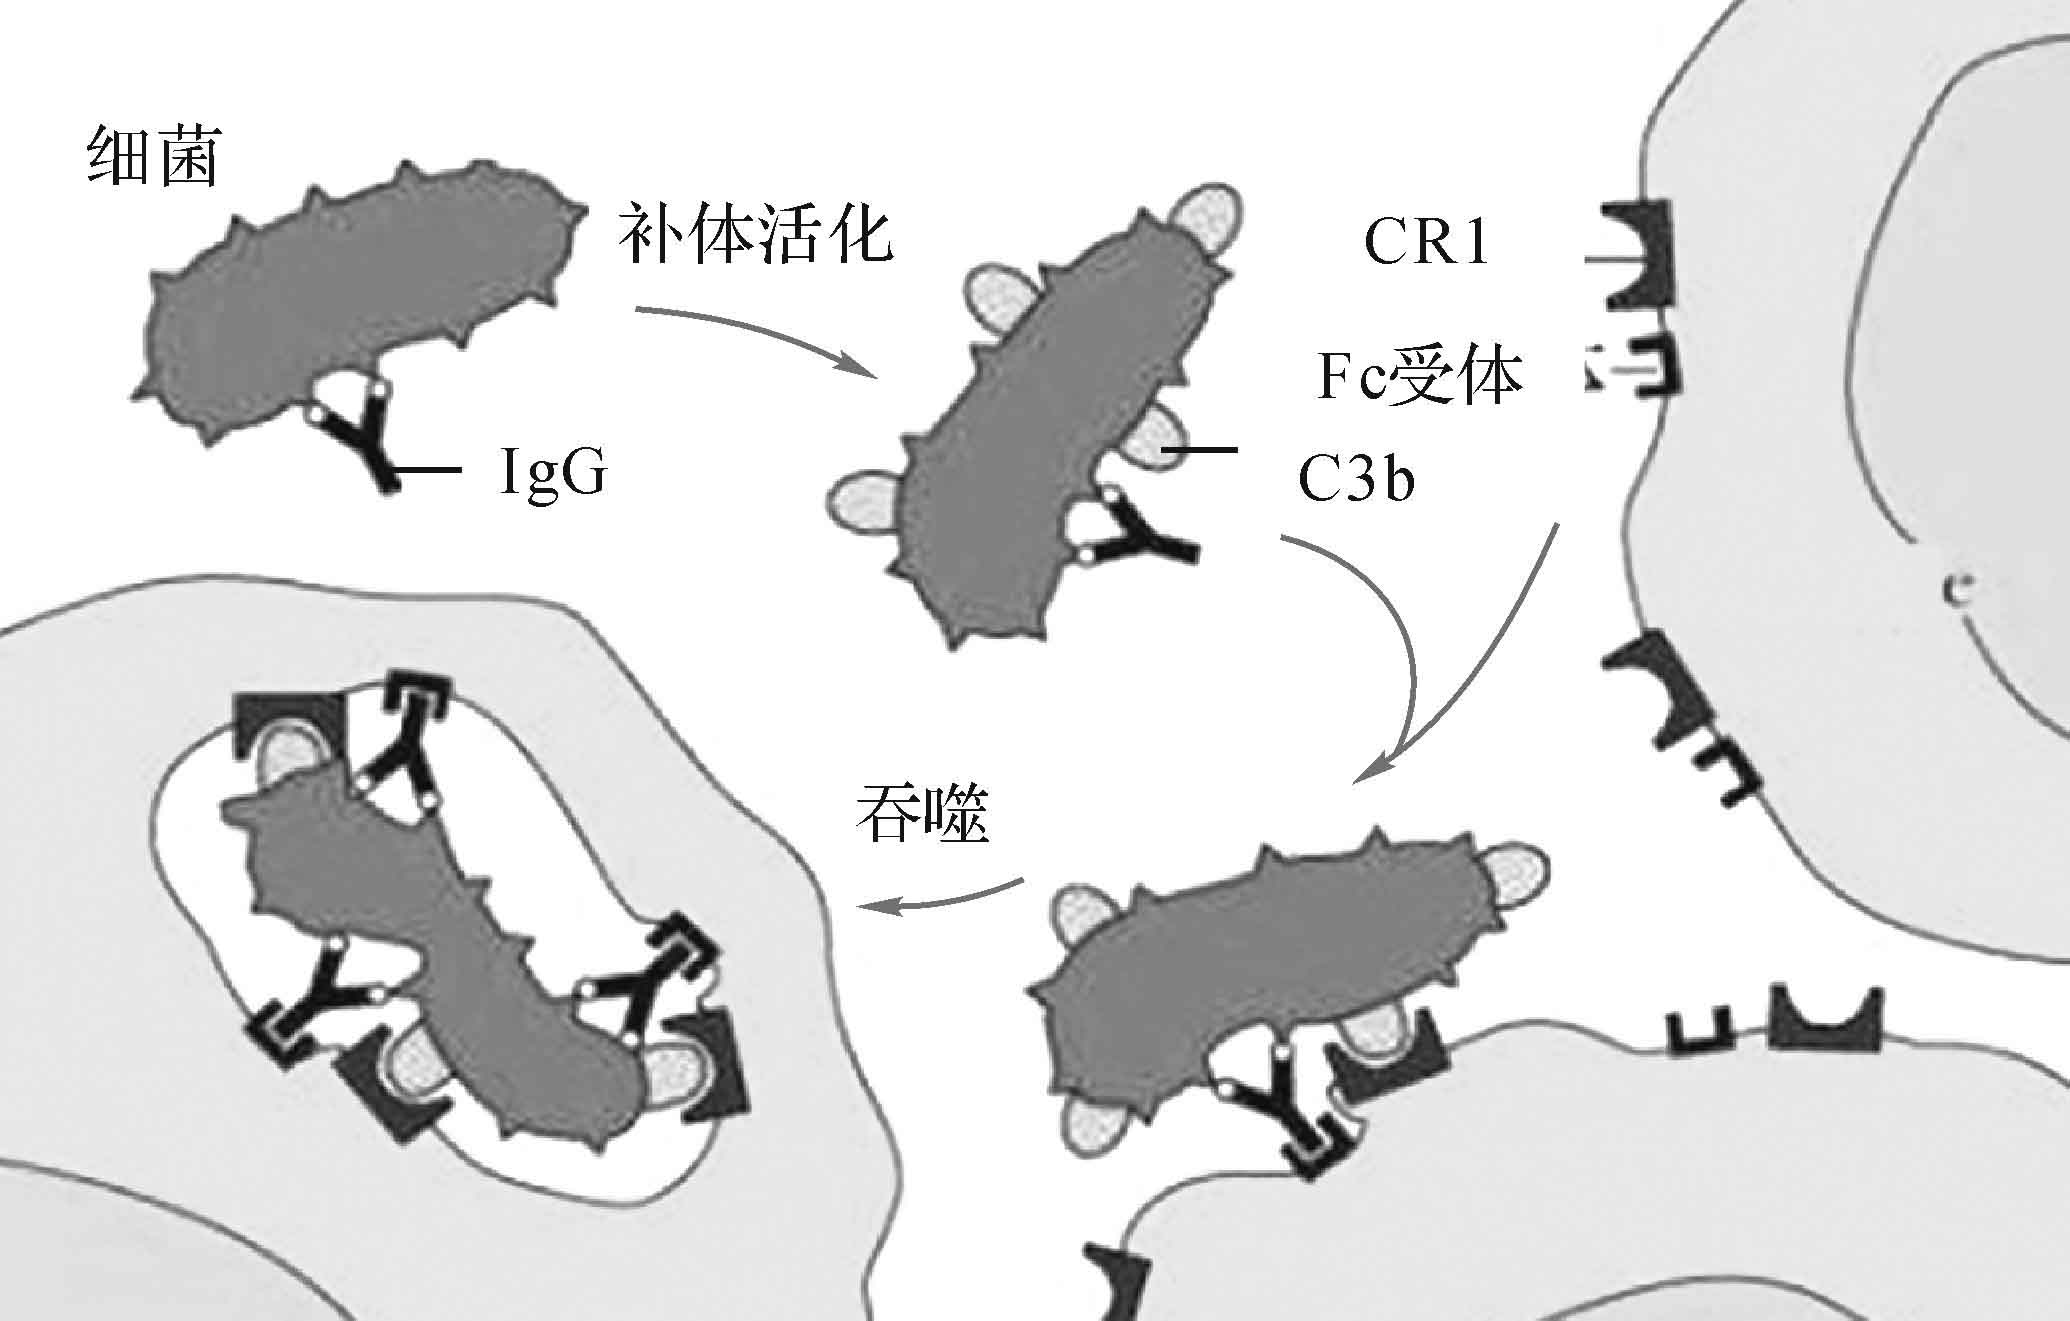
\includegraphics{./images/Image00088.jpg}
 \captionsetup{justification=centering}
 \caption{C3b/CR1促进吞噬细胞的吞噬(调理)作用}
 \label{fig5-10}
  \end{figure} 


\subsection{免疫黏附作用}

\begin{figure}[!htbp]
 \centering
 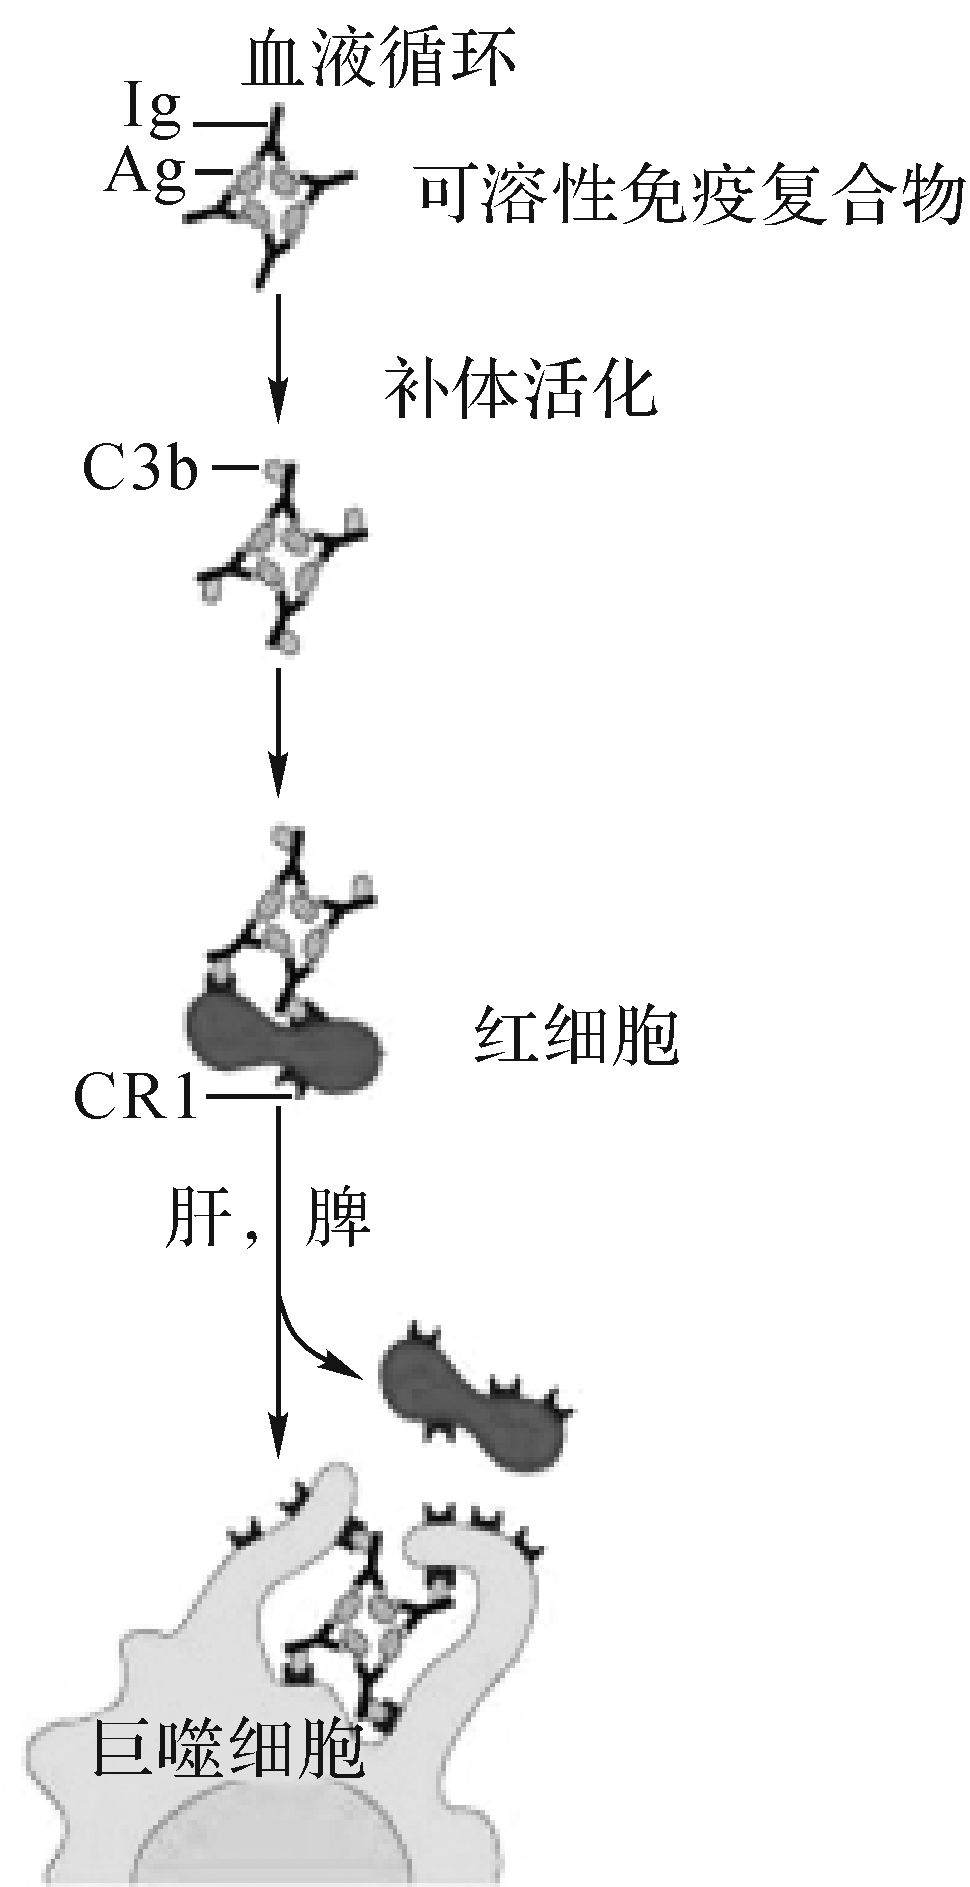
\includegraphics{./images/Image00089.jpg}
 \captionsetup{justification=centering}
 \caption{C3b/CR1介导的免疫黏附作用}
 \label{fig5-11}
  \end{figure} 



可溶性抗原-抗体复合物(如毒素-抗毒素复合物)活化补体后,产生的C3b可共价结合至复合物上,通过C3b与CR1阳性红细胞、血小板黏附,将免疫复合物转移至肝、脾脏内,被巨噬细胞清除,此为免疫黏附(immune
adherent),是机体清除循环免疫复合物的重要机制(图\ref{fig5-11})。


\subsection{炎症介质作用}

C3a和C5a被称为过敏毒素(anaphylatoxin),它们可与肥大细胞或嗜碱粒细胞表面C3aR和C5aR结合,触发靶细胞脱颗粒,释放组胺和其他血管介质,介导局部炎症反应。此外,C5a对中性粒细胞等有很强趋化活性;可诱导中性粒细胞表达黏附分子;刺激中性粒细胞产生氧自由基、前列腺素和花生四烯酸;引起血管扩张、毛细血管通透性增高、平滑肌收缩等。

\noindent\textbf{【理解与思考】}

1.请你以拟人化的方式讲述补体系统的组成与作用。

2.如果病原菌进入机体内,可能遭遇补体怎样的清理?

3.炎症的症状是“红、肿、热、痛”,补体是如何参与其中的?

4.请联系免疫球蛋白的生物学活性阐述补体的作用。

\noindent\textbf{【课外拓展】}

1.补体调节因子如何参与对补体活化或抑制的调控?

2.血清补体水平与疾病有关系吗?

3.补体固有成分、补体受体、补体调节蛋白是如何协调、统一的?

\noindent\textbf{【课程实验与研究】}

1.设计一种实验,检测、测定某种补体成分的作用。

2.请设计一个技术路线,确定补体含量与疾病的关系。

3.要研究某种补体调节蛋白的生物学活性,请设计一种方案。

4.补体调节蛋白CD 46、CD 55和CD 59与胃肠肿瘤相关性如何去验证?

\noindent\textbf{【课程研讨】}

1.补体是如何发现的?其思路对我们科学研究有什么启迪?

2.补体的激活或灭活对维持整个机体内环境的稳定有何作用?试举例阐述机体内环境处于一种动态平衡。

3.在整个非特异性免疫中补体的作用与地位如何?

4.补体与糖尿病血管病变有何关系?

\noindent\textbf{【课后思考】}

1.试比较补体三条激活途径的异同点。

2.补体系统具有哪些生物学功能?

3.补体激活后,可能产生哪些片段?有何生物学作用?

\noindent\textbf{【课外阅读】}

\begin{center}
  \textbf{\Large 衰变加速因子(DAF)与肿瘤治疗}
\end{center}

补体系统的活化过程存在精密的调控机制,主要为:①控制补体活化的启动;②补体活性片段的自发性衰变;③血浆中和细胞膜表面存在多种补体调节蛋白,通过控制级联酶促反应过程中酶活性和MAC组装等关键步骤而发挥调节作用。1993年,Hansch把调节人类补体并阻止组织损伤的蛋白命名为补体调节蛋白,将其分为可溶性及膜结合调节蛋白两大类。它们的主要作用是加速C3/C5转化酶降解和阻碍膜攻击复合物(Membrane
attack
complex,MAC)的形成。可溶性补体调节蛋白以可溶形式存在于血液中,如C1抑制物、H因子、I因子等,可从补体级联反应的多个位点限制补体的活化。膜结合调节蛋白主要表达于细胞膜上,主要包括衰变加速因子(DAF)、膜辅助蛋白(MCP)、同种限制因子等,这些蛋白可保护机体自身细胞免受补体的攻击。

1981年,Weller等从人和豚鼠红细胞基质中分离出了一种单链膜糖蛋白。因其具有促进C3转化酶复合物解离的特性,故命名为衰变加速因子(
Decay accelerating
factor,DAF)。DAF是由4个SCR加上一个S/T(Serine/Threonine)富含区组成,可通过连接一个糖基磷脂酰肌醇(GPI)锚定在细胞膜上,并通过其SCR区域与C4b/C3b结合,加速经典和替代途径C3/C5转化酶的衰变。DAF的生物学活性及生理功能已得到充分证实。它可保护宿主细胞免遭补体介导的溶解破坏。DAF可阻止三种补体激活途径C3和C5转化酶的装配,抑制补体活化过程中多种具有炎症介质作用的活性片段如C3a和C5a的形成,进一步减少中性粒细胞在特定组织器官内的聚集,使已形成的C3、C5转化酶失去稳定性从而减轻免疫损伤。肝脏是合成补体的主要场所,特别是炎症急性期。此时人体如何避免局部高补体浓度的损伤?有研究发现此期的IL-6、IL-1β和TNF-α可稳定提高DAF的转录水平,其蛋白水平的表达与mRNA结果相关,增高的DAF能减少细胞上41\%的C3沉积。与此相似,TNF-α和IFN-γ也可诱导内皮细胞上DAF的表达。进一步实施动物实验证明:体外TNF-α通过PKCPI-3P38MAPK/NF-κB依赖途径上调小鼠内皮细胞DAF转录水平,体内通过构建小鼠肾小球性肾炎模型,发现DAF在肾小球毛细血管的表达水平确实与TNF-α相关。人体能通过上述途径加强对补体激活的抑制作用,提高这些细胞对补体裂解作用的耐受,特别是急慢性炎症反应时,这种调节对维持细胞的完整性和内稳态的平衡起着更重要的作用。

DAF作为一类非谱系的黏附分子在多种细胞上都有不同水平的表达。至今许多学者从转录和蛋白翻译两个水平证明结肠直肠癌、胃癌、卵巢癌、乳腺癌的细胞及甲状腺的髓质、食道癌的鳞状细胞上存在DAF过表达的现象,它的表达量可为正常细胞的4~100倍,而且与肿瘤不良的预后相关,同时在肿瘤的基质中,DAF的沉积量与细胞表面DAF表达量成正比例。除实体瘤外,在血液系统肿瘤中表达DAF的量与正常细胞也有些不同,CML和CLL患者高表达DAF,而ALL患者的表达水平却显著低于正常细胞。

肿瘤细胞上过表达DAF不仅可以保护肿瘤细胞免于被补体裂解,而且它还可以抑制C3b在细胞表面沉积来阻止抗原递呈细胞的吞噬作用。通过K562细胞系进行实验也可以证明,肿瘤细胞上过表达DAF可以使肿瘤耐受NK细胞的杀伤作用。另外,Morgan还提出DAF也许可作为肿瘤细胞上的一个信号分子,促进肿瘤细胞生长。有实验表明,CD97作为DAF的配体在甲状腺肿瘤组织中高表达,它可能参与肿瘤细胞上DAF的信号转导,并与DAF协同作用促进肿瘤细胞黏附和转移。DAF分子的这些作用使肿瘤细胞逃脱机体有效的免疫监视作用,降低抗肿瘤免疫应答,利于肿瘤的生长和转移播散。

基于DAF对肿瘤的作用,进行针对DAF的靶向免疫治疗方法现已备受瞩目。一种方法是构建抗DAF和抗肿瘤特异性抗原的双特异性抗体,但为了避免对正常组织的非特异性影响,肿瘤特异性抗原抗体要求较高的亲和性,而DAF抗体则要求低亲和力。Anti-Ep-CAM-anti-DAF的双特异性抗体可以增加子宫颈癌和结肠癌肿瘤细胞表面的C3沉积。Anti-G250-anti-DAF双特异抗体可提高C5a浓度趋化吞噬细胞,并随着抗体浓度增加最大可提高4倍量的C3沉积,吞噬细胞通过其上的C3受体与肾肿瘤细胞结合,来有效地杀伤肿瘤细胞。另外一种选择则可用抗独特性抗体模拟DAF。来源于结肠癌患者的抗体105AD7不但可以识别抗体791T/36(DAF抗体),而且可以模拟DAF。用105AD7免疫大鼠和小鼠都能产生针对DAF的抗体。近期研究还表明,在肿瘤切除前接受105AD7免疫的患者局部CD4、CD8和CD56细胞浸润增加并且肿瘤凋亡数量也增加。现已发现无GPI锚的DAF出现在结肠癌患者粪便中,并建议用粪便中DAF含量作为结肠癌诊断的指标。最近研究指出同一患者进行两次粪便样本检测,可以显著提高结肠癌疾病诊断的灵敏性而不降低特异性。

\begin{center}
  \textbf{\Large 补体片段C4d病理学研究进展}
\end{center}

补体片段C4d主要参与体液免疫反应。近年来,C4d在病理学中应用研究方面取得了一些重要进展,并成为了一个新的研究热点,日益受到人们重视。现就C4d在器官移植排斥反应的诊断、指导治疗及判断预后,自身免疫性疾病、妊娠性肾病和淋巴瘤中的意义进行综述。

1 C4d概述

补体片段C4d是补体经典活化途径中C4裂解以后的产物,相对分子质量约为42×10\textsuperscript{3}
。C4是补体系统中含量较高的补体,仅次于C3。在体液排异中,抗原抗体结合使得补体经典途径被激活,抗原抗体复合物活化C4,被活化的C4水解为CD4一个大分子片段C4b和一个小分子片段C4a,后者释放入液相。C4b的α链断端上暴露的活性硫酯键高度不稳定,能与附近的含氨基酸或羟基的分子共价结合形成酰胺键或者酯键,而未结合的C4b很快被灭活。共价结合的C4b随后水解为C4c和C4d,小片段C4c释放入液相后被机体清除掉,而包含硫酯位点的C4d能与毛细血管基膜Ⅳ型胶原以及内皮细胞共价结合并较持久地存在,使得其容易得到检测。

2 C4d在器官移植中的应用

2.1 C4d与移植肾急性排斥反应

移植肾急性排斥反应可以由细胞介导的免疫引起,也可以由抗体介导的体液免疫引起。前者称为急性细胞性排斥,常发生在移植术后1个月内;后者称为急性体液性排斥,一般在移植后1~12周内出现。研究表明,移植肾急性体液性排斥可出现肾小管周围毛细血管的C4d沉积,借助C4d可以区分急性细胞性排斥和急性体液性排斥,且较以往的标准更特异、更敏感。移植肾排斥新分类已将C4d作为一项重要的诊断指标,甚至在缺乏形态学的依据时亦然。C4d亦可用于指导治疗及提示预后。有研究显示,C4d阳性组无论是在激素治疗抗药性还是移植肾丢失率都高于阴性组,因此可望作为一个有效的预后指标。Vargha等对36例移植肾患儿的回顾性研究发现,移植肾C4d阳性可能提示预后较差,且使用免疫抑制疗法效果欠佳。最近一项对C4d阳性移植肾急性体液性排斥免疫抑制治疗的研究结果显示,联合应用免疫吸附以及他克莫司和霉酚酸酯用于治疗C4d阳性激素抵抗型急性排斥反应,可能是比较安全和经济的治疗方案。

2.2 C4d与移植肾慢性排斥反应及慢性移植性肾病

慢性移植性肾病概念上有别于移植肾慢性排斥反应,前者更加强调了非免疫因素引起的肾功能损害,而后者则强调免疫因素所致移植肾功能减退。慢性排斥反应是术后6~12个月肾功能不全的常见原因,也是后期肾丢失的主要原因。由于形态学观察上的局限性,需要一种更加特异和可靠的方法鉴别慢性排斥反应和其他原因引起的移植肾慢性失功。以往的研究表明,一部分慢性排斥是抗体介导的,而且肾小管周围毛细血管C4d沉积可以区分慢性排斥反应与非特异性慢性移植性肾病。Regele等观察了213例慢性移植肾损伤的形态学特征,其中73例(34\%)肾小管周围毛细血管有C4d沉积,进一步支持了部分慢性排斥反应是由抗体介导的这一观点。此外,不仅肾小管周围毛细血管有C4d沉积,而且肾小球毛细血管也有C4d沉积,但不具有特异性,可以看作是免疫介导损伤的一种表现。然而,最近研究表明,在慢性移植性肾病患者中有30\%的病例有肾小管周围毛细血管C4d沉积,这使得C4d与慢性排斥反应和慢性移植性肾病之间的关系更加扑朔迷离,需要进一步深入研究。

2.3 C4d与肝移植急性排斥反应

和肾移植排斥反应一样,肝移植细胞排斥反应也会同时伴有体液排斥反应。有研究发现,在急性细胞排斥反应中,69.2\%的肝移植标本在肝小叶汇管区小血管内皮细胞及肝血窦壁上有C4d的沉积,33.3\%移植后乙肝复发的标本中仅汇管区小血管内皮细胞上有C4d的沉积,而无肝血窦壁上C4d的沉积。这说明C4d在肝血窦壁上的沉积可能是肝移植急性排斥反应的一个比较特异的免疫组化指标。以后的研究不仅进一步支持了以上的观点,并且提示C4d还可能用于肝移植急性排斥反应与丙型肝炎的鉴别诊断。

2.4 C4d与心脏移植排斥反应

关于C4d与心脏移植排斥的报道要早于肝脏移植排斥中C4d的发现,但是C4d在心脏移植排斥中的应用价值目前研究还不够深入。心脏移植患者心内膜血管壁上有C4d沉积,说明体液性排斥也会参与心脏移植排斥反应。因此,配合使用C4d、C3d、免疫球蛋白和C1q等抗体可以提高对心脏移植体液排斥反应的诊断率。但是,C4d的沉积有时并不是很牢固,可以在几天至几周内出现沉积减少或被清除掉的现象,其具体原因还不清楚。

2.5 C4d与肺移植排斥反应

移植后的排斥反应和闭塞性细支气管炎是器官丢失的常见原因。尽管补体系统的激活在排斥反应中起一定的作用,但是关于C4d在肺移植排斥反应中的作用目前还存在争论。有研究认为,C4d在肺实质中的沉积可以是闭塞性细支气管炎的一个比较特异的表现,并可以作为慢性肺功能障碍的一个标志。小鼠移植肺动物模型中也观察到在急性排斥反应中有C4d的沉积。但是,Wallace等提出,C4d在移植肺活检标本中的沉积不具有特异性,不能够区分急、慢性细胞及体液性排斥反应。因此,C4d在肺移植排斥反应的作用尚不是很明了,待进一步的研究。

2.6 C4d在胰腺移植排斥反应中的应用

目前,关于抗体介导胰腺移植排斥反应的报道很少。Melcher等首先报道1例患者在进行了胰腺、肾脏联合移植术后1个月出现抗体介导的细胞排斥反应。该患者血清淀粉酶和血糖升高,胰腺活检显示,腺泡间毛细血管壁C4d沉积。但这种沉积在病理学中意义以及在临床上的应用价值还没有相关报道。

3 C4d在自身免疫性疾病中的应用

C4d与自身免疫性疾病的研究目前主要集中在系统性红斑狼疮(systemiclupuserythematosus,SLE)和狼疮性肾炎方面。目前临床对于SLE的诊断、疾病活动度、病情进展、治疗效果以及预后的估计主要用血清学标记,如:抗DNA抗体、抗C1q抗体等,并具有较高的敏感性和特异性。有研究显示,抗C1q抗体与狼疮性肾炎的活动性有关,敏感度为44\%~100\%,特异度为70\%~92\%。但是单一的检测指标容易出现假阴性,需要多种指标联合应用,互相补充,减少假阴性。

为了寻找更具特异性和敏感性的检测指标,许多学者又进行了大量的研究。Manzi等首次发现,SLE患者较其他自身免疫疾病患者或健康组具有很高水平的红细胞和较低水平的补体受体1。与健康组相比,红细胞Π补体受体1检测的敏感度为81\%,特异度为91\%;与其他自身免疫疾病相比,检测的敏感度为72\%,特异度为79\%。而同期观察的SLE患者中只有47\%证实抗DNA抗体阳性。这些数据充分显示,红细胞Π补体受体1水平对于SLE具有更高的敏感性和特异性,有可能成为狼疮新的诊断标志物。另一组研究人员应用流式细胞仪研究了网织红细胞C4d,不仅明确检测到了网织红细胞C4d,而且其敏感性和特异性均优于SELENA2SLEDAI和SLAM标准。他们推测,当网织红细胞从骨髓中产生,就立即与C4d结合,进行一定量的补体激活,进而可以反映SLE患者疾病活动度。SLE患者不仅红细胞C4d表达具有相对特异性,而且血小板C4d的表达也同样具有特异性,甚至还要高于红细胞。Navratil等发现,SLE患者血小板C4d阳性明显,并均质性地沉积在血小板膜表面。与健康组相比,SLE患者血小板C4d特异度为100\%,而和其他疾病患者相比,特异度为98\%。在横向比较分析中发现,血小板C4d与狼疮抗凝物、IgG、IgM以及抗心磷脂抗体具有相关性。此外,血小板C4d还与低血清C4、血沉升高以及红细胞具有相关性。以上结果均表明,血小板C4d与SLE疾病活动度相关,并有可能成为SLE活动度有效的监测指标之一。

4 C4d与淋巴瘤

早在1989年就发现淋巴滤泡生发中心形成过程中有大量补体成分沉积。近年来的研究证明,淋巴滤泡生发中心补体成分的沉积与滤泡树突细胞密切相关,补体成分中C4d的表达最强,因此可以用C4d作为代表性的标志,观察淋巴生发中心补体激活的状态。在滤泡性淋巴瘤中,C4d沉积围绕在瘤性滤泡中的滤泡树突状细胞周围,而在黏膜相关淋巴瘤中,C4d沉积主要在部分植入滤泡的周边区域。而在其他类型的淋巴瘤(如弥漫大B细胞淋巴瘤、套细胞淋巴瘤、小B细胞性淋巴瘤、T细胞性淋巴瘤、外周T细胞性淋巴瘤)中,则没有C4d的沉积。因此,C4d可能作为一种特异性的生物学标志用于淋巴瘤的鉴别诊断。

5 C4d与妊娠性肾病

Joyama等曾报道1例先兆子痫患者在肾小球毛细血管内皮下上有C4d和C4b结合蛋白的沉积,同时,免疫组织化学还显示有C3d和S蛋白的沉积。提示补体C4的激活过程与C4b结合蛋白和S蛋白参与的补体调节过程在先兆子痫发病过程中可能起一定的作用。宋屿娜等也发现,l4例临床诊断为先兆子痫的妊娠性肾病患者除肾小球血管壁C4d均呈强阳性,系膜区未见表达,C4c也呈强阳性,免疫球蛋白沉积少或缺乏。而膜增殖性肾炎组的系膜区和血管壁均有C4d沉积,同时还伴有大量各种免疫球蛋白的沉积。借此可用于膜增殖性肾炎的鉴别诊断。但是这种特殊的免疫病理改变原因仍不清楚。这种C4d沿肾小球血管壁大量沉积的原因显然不能用免疫球蛋白沉积后激活补体系统来解释。由此推测,这些C4d和C4c可能是在血液中被激活后,再通过肾小球毛细血管壁过滤时沉积下来的。

6 问题与展望

综上所述,随着对补体片段C4d研究的深入,人们逐渐认识到C4d可以作为一种有用的生物学指标,用于对疾病的诊断、指导治疗、判断预后以及反映疾病的活动度。但是,其中仍然还有许多问题尚待解决和探索,如C4d在肾脏不同部位的沉积与肾脏损伤的关系,C4d与其他自身免疫性疾病的关系以及补体与免疫细胞、免疫系统的关系等。

\begin{center}
  \textbf{\Large 免疫过程中一种重要的补体受体}
\end{center}

枯否细胞(Kupffer
cells,KC)是一种肝脏巨噬细胞,具有很强的吞噬功能,可以降解已经衰败的蛋白质和脂质,在清理循环系统中补体包裹的微粒(complement-coated
particles)方面作用重大,但是一直以来研究人员都没有发现这个过程中的补体受体(complement
receptors)。来自加州旧金山南部(South San
Francisco,CA)的Genentech基因科技公司的研究人员发现并确认了一组免疫球蛋白超家族补体受体CRIg,为研究免疫学疾病提供了重要信息。

在血液或体液内除Ig分子外,还发现另一组参与免疫效应的大分子,称为补体分子。早在19世纪末,发现在新鲜免疫血清内加入相应细菌,无论进行体内或体外实验,均证明可以将细菌溶解,将这种现象称之为免疫溶菌现象。进一步证明免疫血清中含有两种物质与溶菌现象有关,即对热稳定的组分称为杀菌素,即抗体。其后又证实了抗各种动物红细胞的抗体加入补体成分亦可引起红细胞的溶解现象。自此建立了早期的补体概念。即补体为正常血清中的单一组分,它可被抗原与抗体形成的复合物所活化,产生溶菌和溶细胞现象------单独的抗体或补体均不能引起细胞溶解现象。

补体系统在清除病原菌、免疫复合物以及循环系统中的凋亡细胞等方面都起着重要作用,这一作用主要是通过在噬菌细胞(phagocytic
cells)表面的补体受体靶定包裹在上述这些微粒外面的补体片段来完成的。虽然目前已经了解KC这种巨噬细胞可以参与这个过程,但是具体补体受体并未被发现。Genentech的研究人员发现免疫球蛋白超家族补体受体CRIg可以结合C3b和iC3b(C3b配体)补体,并且KC细胞结合C3微粒的噬菌作用需要有CRIg的表达。反过来,研究人员也发现CRIg缺陷型小鼠不能进行有效的C3补体结合的微粒清除,从而导致小鼠的感染和致死。这些都说明了CRIg在C3补体介导的噬菌过程中的重要作用,也为进一步研究补体系统以及相关免疫学疾病提供了重要信息。

